\begin{itemize}
    \item Beschreibt die Grundüberlegungen der realisierten Lösung (Konstruktion/Entwurf) und die Realisierung als Simulation, als Prototyp oder als Software-Komponente etc.
    \item Hier beschreiben Sie Ihre gemachte Arbeit. Dazu braucht es eine Beschreibung des Vorgehens, aller Arbeitsschritte usw.
    \item (Definiert Messgrössen, beschreibt Mess- oder Versuchsaufbau, beschreibt und dokumentiert Durchführung der Messungen/Versuche)
    \item Bildmaterial erleichtert das Verständnis.
    \item (Experimente)
    \item Immer mit Aufbau und Vorgehen; Bildmaterial erleichtert das Verständnis.
    \item (Lösungsweg)
    \item Inkl. theoretische Herleitung der Lösung
    \item (Modell)
    \item (Eingesetzte Software)
    \item Die Funktionen von verwendeten Computerprogrammen zu Simulationszwecken, Berechnungen etc. sollen beschrieben werden. Dies soll aber in Worten, Formeln und geeigneten Darstellungen (z.B. Fluss- diagrammen) geschehen. Allfälliger Programmcode ist in einem Anhang zu dokumentieren.
    \item (Tests und Validierung)
\end{itemize}

\textbf{Marco's Proposal}
\begin{itemize}
    \item Anfangs High Level Overview Mischung, Kapitel ersichtlich was kommt Flussdiagram (um dieses haben wir dann die Prozessmethoden)
    \item Vorgehensmethode => Kanban und Scrum, maybe V-Model?
    \item Setup technisch, lokale Linux VM, ROS Installation, VS Code als IDE, GitHub Repos, GitHub Actions CI/CD (maybe?), Deployment Architektur
    \item Overview Architektur ROS und Code, Grundüberlegung => Path Planning Package in ROS, Prototyp Architektur zeigen, Explo und Opt Algos, erhaltet Input und sendet Input
    \item Messages (interfaces und fszhaw msgs) (System aussen)
    \item Path Planner Node
    \item Exploration Algorithm
    \item Optimization Service Node
    \item Optimization Algorithm
    \item Verifikation und Validierungen (Code Reviews, Fehlerfälle: Cones gehen verloren, Cones andere Seite entdeckt, allg Fehlerannahmen)
    \item Testing mit Maps, Cone Publisher und Planned Trajectory Subscriber (mocks), utils wie track plotter, trackconfig
    \item Setup eher im Projektanhang: Weekly meetings, Review every other week, Mitarbeit mit anderen BA Teams in Driverless und gesamt Verein (Working Saturday, Hilfe im Workshop, Ausstellung Conecto ZHAW)
    \item In Resultate Kapitel, Vergleich erste Algorithmen und Versuche: erste Überlegungen und Tests, alter path planner zhaw, dann densify und interpolate, rrt max hamburg, komplexer algo à la ultimate und dann jetzige implementation, zuerst was hat eth mit mpcc, dann global racetrajectory von tumftm
\end{itemize}

This chapter describes which approaches and methods have been used to solve the problem to find algorithms which calculate the optimum path on a racetrack. The V-Model was used to plan the overall project as shown in figure \ref{fig:High Level Project Overview}. Scrum was used for the meetings that were held with the supervisors and the driverless team to accomplish the planning of the sprints. Further explanation on the planning process is described in the section \ref{sec:Planning Methods}. After the planning section, the development environment is described in section \ref{sec:Development Environment}. Then an introduction to the architecture design of the Path Planning component is explained in section \ref{sec:Path Planning Component Architecture}. The algorithms are explained in section \ref{sec:Exploration Algorithm} for the exploration and section \ref{sec:Optimization Algorithm} for the optimization algorithm. Lastly the integration and verification process is described in section \ref{sec:Integration and Verification}.

\begin{figure}[H]
    \centering
    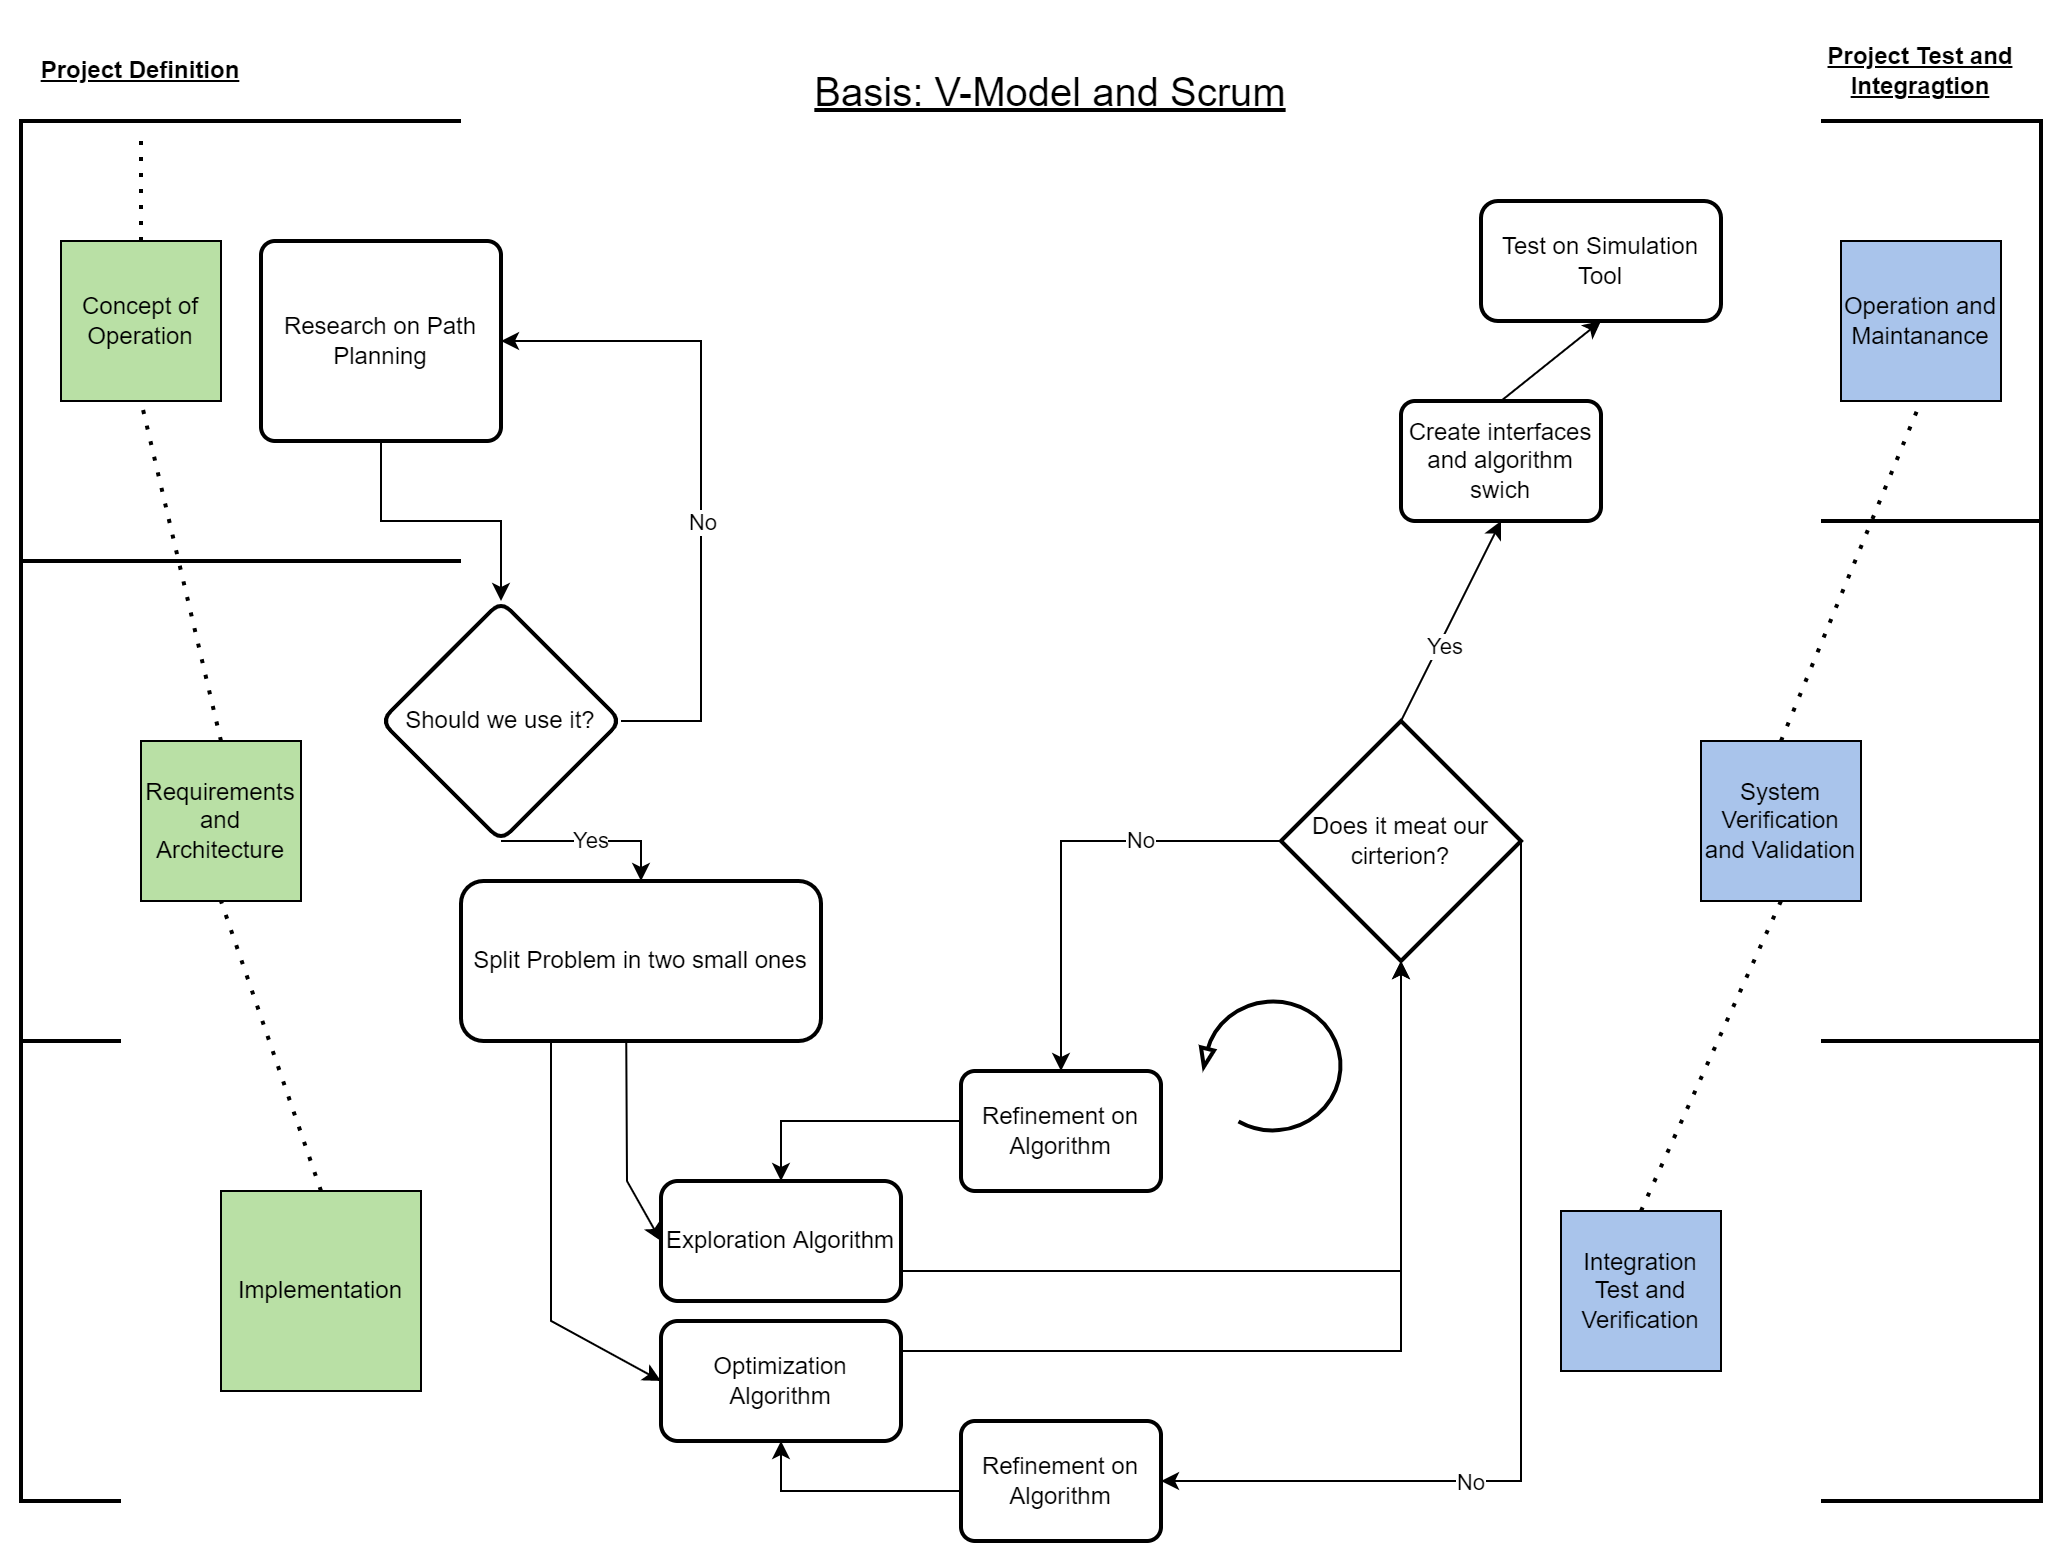
\includegraphics[width=\columnwidth]{High_Level_Project_Overview.png}
    \caption{The high level project overview gives an illustration which approaches and methods have been used to realize the project.}
    \label{fig:High Level Project Overview}
\end{figure}

\section{Planning Methods} \label{sec:Planning Methods}
To accomplish complex tasks in a team or alone there has to be a certain plan. In modern Software Engineering the method Scrum is very common as an agile planning method. As for an overall plan the V-Model was used.

\subsection{V-Model} \label{sec:Planning Method: V-Model}
The V-Model consists of several stages as shown in figure \ref{fig:V-Model}.
\begin{figure}[H]
    \centering
    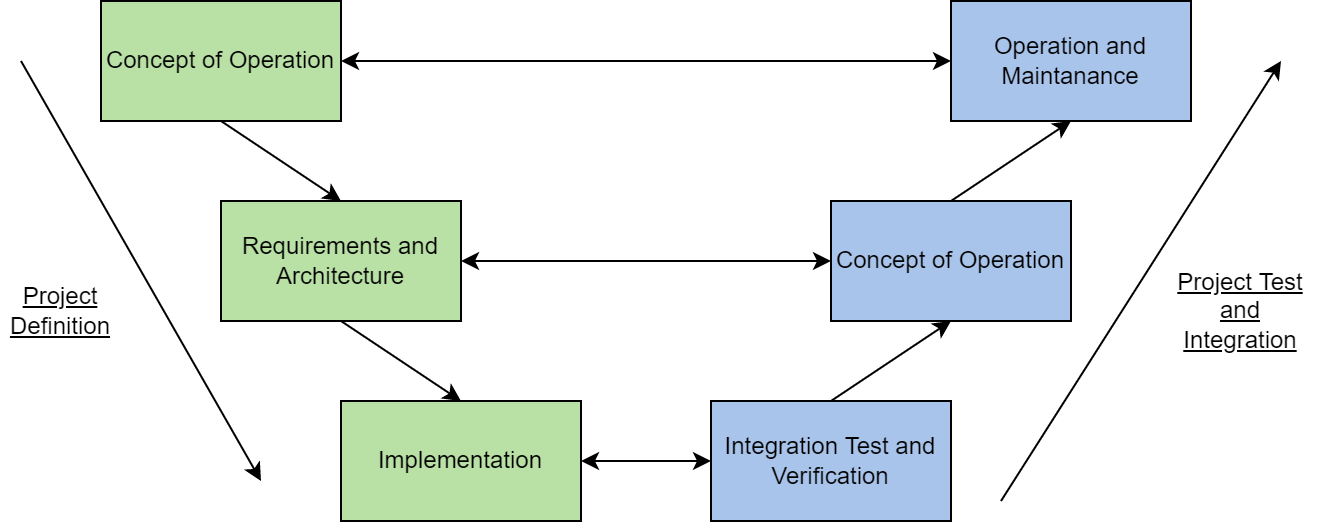
\includegraphics[width=\columnwidth]{V-Model.png}
    \caption{The V-Model helps in an IT-Project to have a focus on planning and implementation while reflecting and testing the program.}
    \label{fig:V-Model}
\end{figure}

Starting with the concept of operation stage. In this stage the plan is made and research is conducted. Second the requirements and architecture is decided. This covers the process of building a development system that is near to the production environment. In this project the production system is the NVIDIA Jetson and the development system the \acrlong{vm}. Splitting up the problem to find an optimum path into two smaller ones like the exploration and optimization algorithm helped to divide the workload and having the four eye principle on each other's code. The last part covers the implementation of the algorithms in the development environment and testing it. At the same time test definition on how to test the algorithms and how to verify a good one has to be done. The integration test and verification is covered in chapter \ref{ch:Results}. The concept of Operation process consists of the evaluation of the algorithms if they fit the criterion. Lastly the operation and maintenance phase deals with the integration of the algorithm into the production system. This is as well the combination of the exploration and optimization algorithm while using interfaces.

\subsection{Scrum} \label{sec:Planning Method: Scrum}
To ensure the communication between supervisors and developers Scrum was used. To get a deeper understanding how Scrum works an explanation in the appendix under \ref{sec:Scrum}. Weekly meetings where held with supervisors and biweekly meetings with the driverless team. In addition, the team itself held a meeting on a weekly basis as well. From the meeting notes user stories were created to translate the stories into code. Before the weekly meeting with the supervisors an e-mail is sent which covered the tasks that have been done in the past week, the task for the week after and problems the team faced during development.

\subsubsection{Kanban Board} \label{sec:Kanban Board}
The kanban board helps to organize the user stories and to prioritize the stories in the development process. In addition, another kanban board was made to write the thesis. As shown in figure \ref{fig:Kanban Board Path Planning} there are four columns. The ``To Do'' list with all the ideas and inputs from supervisors. The ``In progress'' list shows the current tasks and the ``Review in progress'' is for the other team member to review the code. Finally, the ``Done'' column illustrates the finished tasks.
\begin{figure}[H]
    \centering
    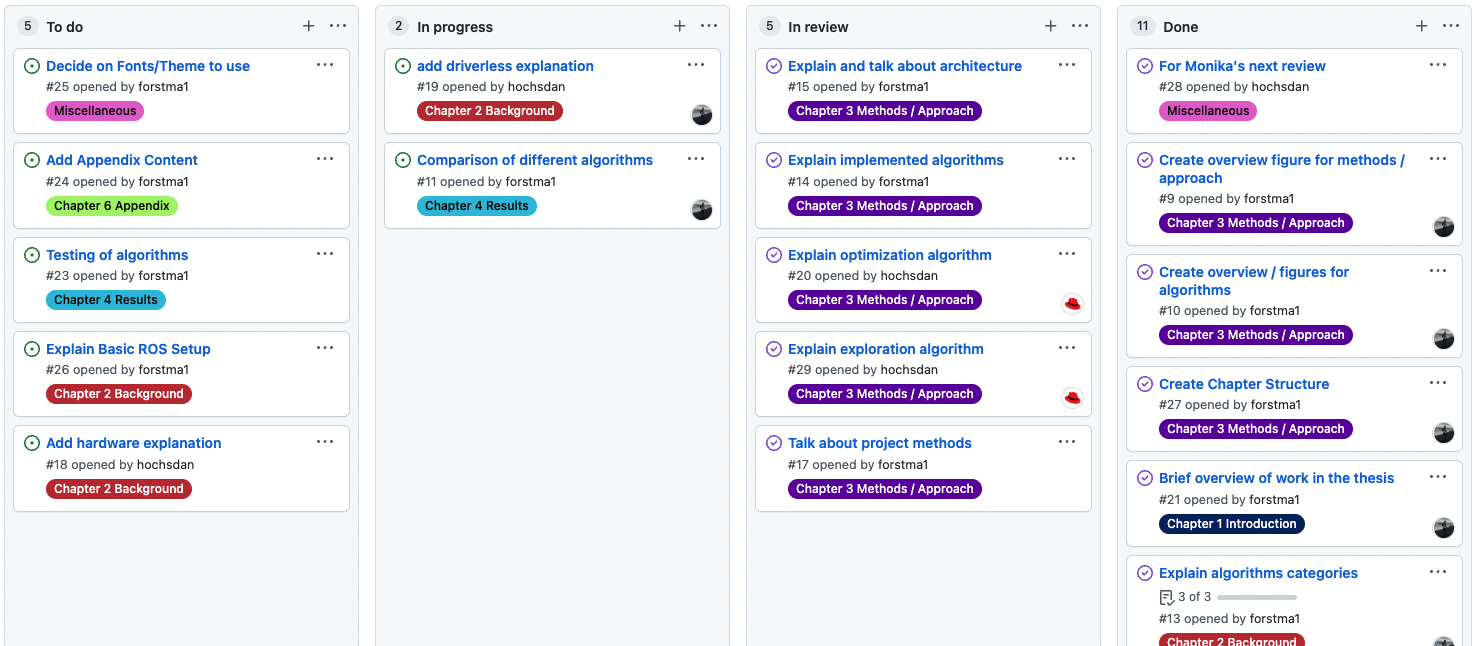
\includegraphics[width=\columnwidth]{Kanban_Board_Path_Planning.PNG}
    \caption{The Kanban Board helps to organize the user stories to see who is working on which story.}
    \label{fig:Kanban Board Path Planning}
\end{figure}

\section{Development Environment} \label{sec:Development Environment}

There are different methods to build a development environment. An easy way to get started is to build a relatively similar system like the one which is running on the NVIDIA Jetson computer. This computer will be used in the real car. A \acrlong{vm} (\acrshort{vm}) is a piece of software that can emulate hardware and encapsulates an operating system from the host operating system, that is running on hardware. Figure \ref{fig:Development Architecture} illustrates the architecture that is used for developing.

\begin{figure}[H]
    \centering
    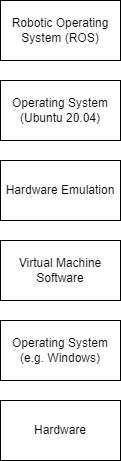
\includegraphics[width=2cm]{Development_Architecture.jpg}
    \caption{The development architecture consists of various levels: the hardware, the host operating system, the \acrlong{vm}, the operating system on the \acrshort{vm} and the \acrlong{ros}.}
    \label{fig:Development Architecture}
\end{figure}

On the NVIDIA Jetson computer an Ubuntu 20.04 operating system was installed. This is the reason why Ubuntu 20.04 is used on the development environment. An installation guide for how to install Ubuntu 20.04 in a \acrlong{vm} is found Cloud Linux Tech. \cite{cloudlinuxtech_install_ubuntu_2004}

The work done in this thesis have been done using the ROS 2 release 'Foxy Fitzroy', released on June 5th, 2020. This release will be supported till the end of May 2023. \cite{ros2_releases_and_target_platforms}

\subsection{Integrated Development Environment (IDE) and Version Control} \label{sec:Integrated Development Environment (IDE) and Version Control}
For developing the \acrshort{ros} node an Integrated Development Environment (IDE) was used called Visual Studio Code. This IDE has the functionality to do syntax checking on the python and C++ code. Further on the IDE was used to write the thesis in Latex as an extension for building PDF files via Latex files can be installed. For both the code and the thesis a separate GIT Repository for version control was created. The version control system helps to develop in a software engineering team to follow changes on the code and in case of any problem it can be jumped back to an older code. The GIT server which was used is \href{https://github.zhaw.ch}{github.zhaw.ch}.

\section{Path Planning Component Architecture} \label{sec:Path Planning Component Architecture}
In this section, an overview on the Path Planning component will be given. As seen in the component Autonomous System Component diagram \ref{fig:AS Component Diagram}, the Path Planner will receive it's inputs by Perception (detected cones) and Localization/Odometry (current position) via the Mapping, and send it's output (planned path) to the Autopilot component.

The path planning component primarily consists of two \acrshort{ros} nodes: The 'Path Planner' node and the 'Optimization Service' node, as seen in figure \ref{fig:Path Planning ROS Architecture}.
\begin{figure}[H]
    \centering
    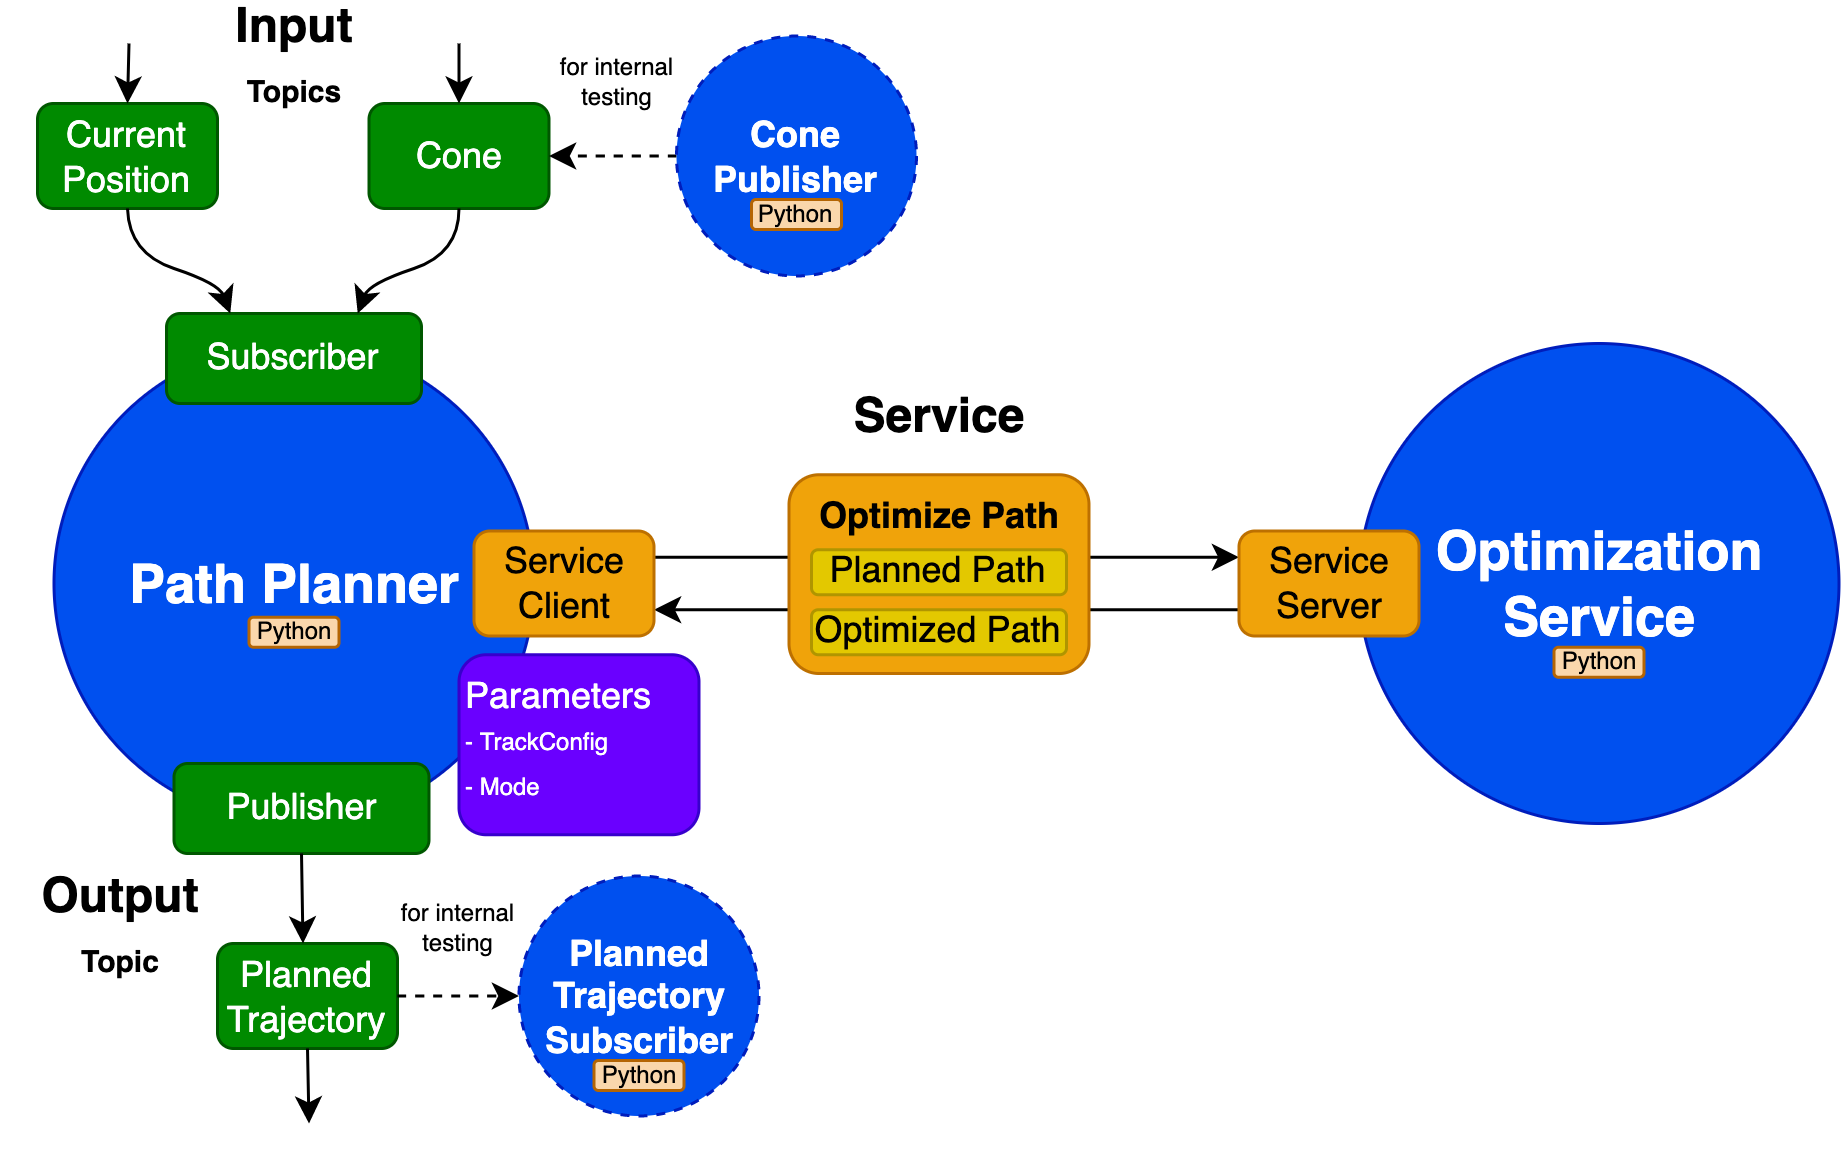
\includegraphics[width=\columnwidth]{Path_Planning_ROS_Architecture.png}
    \caption{The high-level ROS overview of the path planning package, consisting of several nodes and takes advantage of topics and services.}
    \label{fig:Path Planning ROS Architecture}
\end{figure}

The Path Planner node can be seen as the brain of the planner, as it handles both the flow of the data and the management of the different algorithms. It itself subscribes on the inputs and publishes the output via \acrshort{ros} topics. While the car's current position is received by the 'Current Position' topic, the latest detected cone is received by the 'Cone' topic, and the final planned path is then published via the 'Planned Trajectory' topic. The planner will calculate the path for the vehicle using the custom made 'Exploration Algorithm', which will be explained in more detail in section \ref{sec:Exploration Algorithm}. Furthermore, the node holds several configuration parameters regarding the algorithm mode, track configuration and more.

The Path Planner requests the calculation of the optimized path to the Optimization Service. Communication with the service occurs through the 'Optimize Path' \acrshort{ros} service. While the Optimization Service calculates the optimized racing line for the given track, the Path Planner will still continue to calculate the path using the exploration algorithm. The Path Planner will switch to publishing the optimized path after it receives the response from the service.

For testing the package locally in Python, two additional \acrshort{ros} nodes where created: The 'Cone Publisher', for mocking the publishing of cones, and the 'Planned Trajectory Subscriber', for receiving the published trajectories by the planner.

The base structure of the Autonomous System was already defined by the team (see figure \ref{fig:AS Component Diagram}) before work on the thesis even began, hence it was clear on how the structure of the Path Planner would vaguely look like. Receiving detected cones from Perception and receiving the current position from Localization, calculating the path with that data, and then sending that to the next part of the system, an early draft of the planner can be seen in figure \ref{fig:Path Planning ROS Architecture Draft}.
\begin{figure}[H]
    \centering
    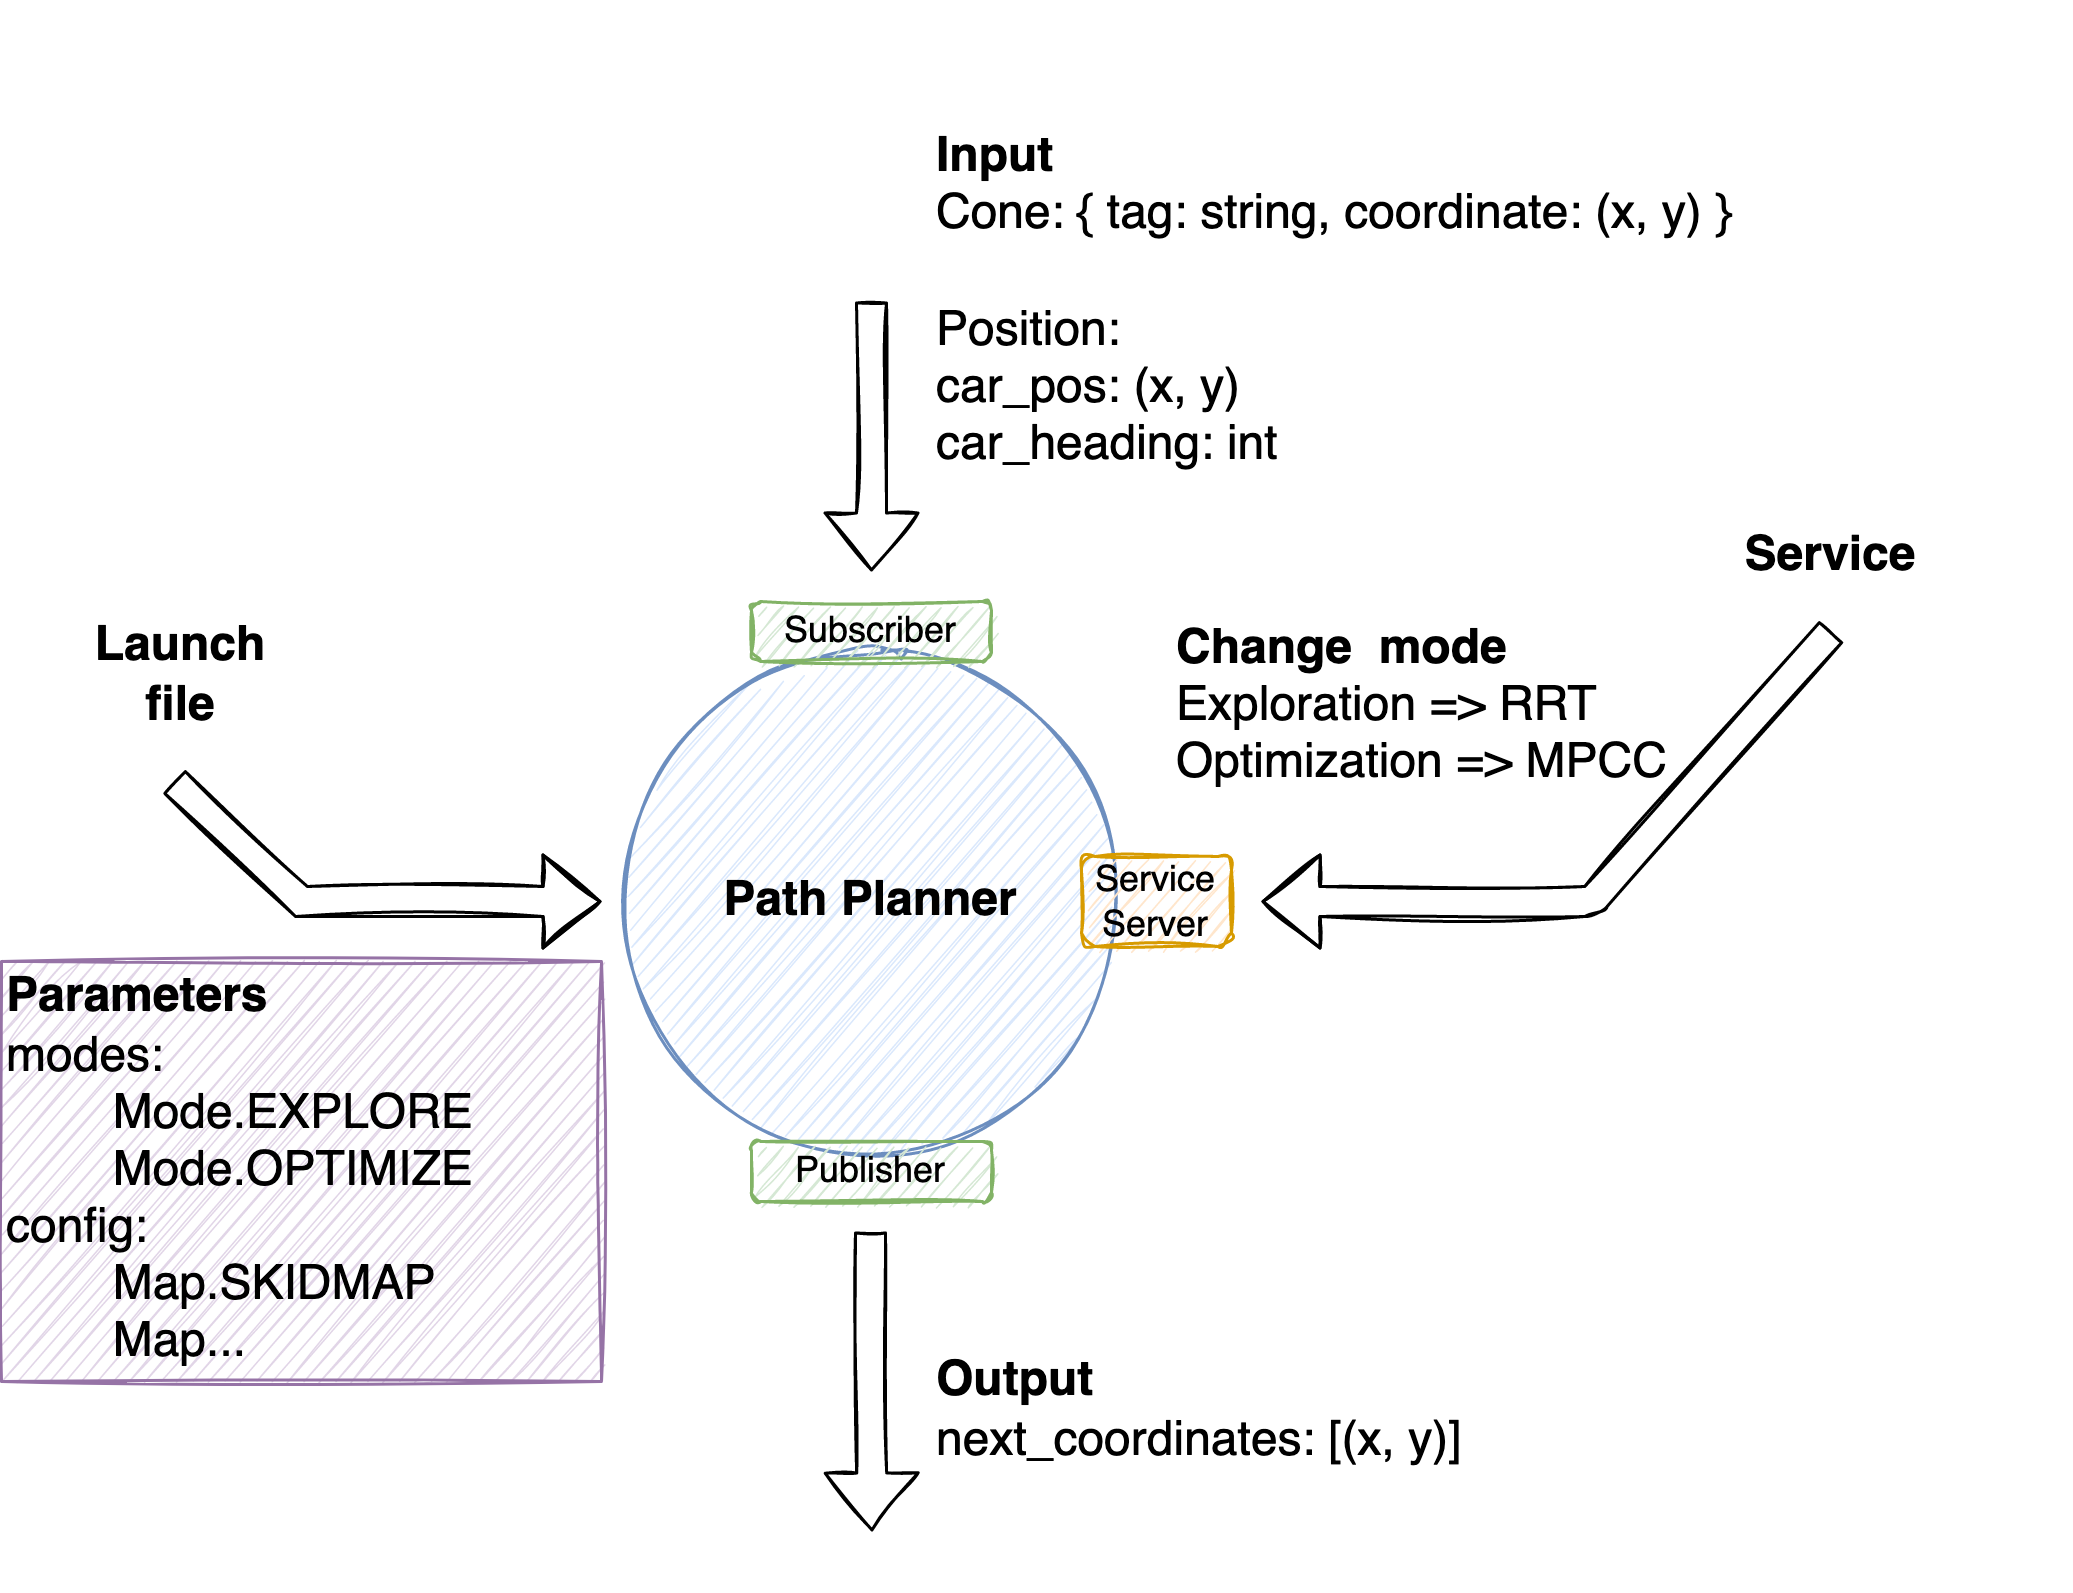
\includegraphics[width=\columnwidth]{Path_Planning_ROS_Architecture_Draft.png}
    \caption{An early draft of the ROS architecture of the path planner.}
    \label{fig:Path Planning ROS Architecture Draft}
\end{figure}

\subsection{Custom ROS Messages} \label{sec:Custom ROS Messages}
As seen in section \ref{sec:Zurich UAS Racing Autonomous System}, for the Autonomous System to fully function, different components developed by different people will have to work together. To enable smooth communication between these different components via the \acrlong{ros}, a set of default \acrshort{ros} messages were defined by the team as seen in figure \ref{fig:Path Planning ROS Messages}. For \acrshort{ros} communication inside of the Path Planning component itself, another package containing \acrshort{ros} messages was created.
\begin{figure}[H]
    \centering
    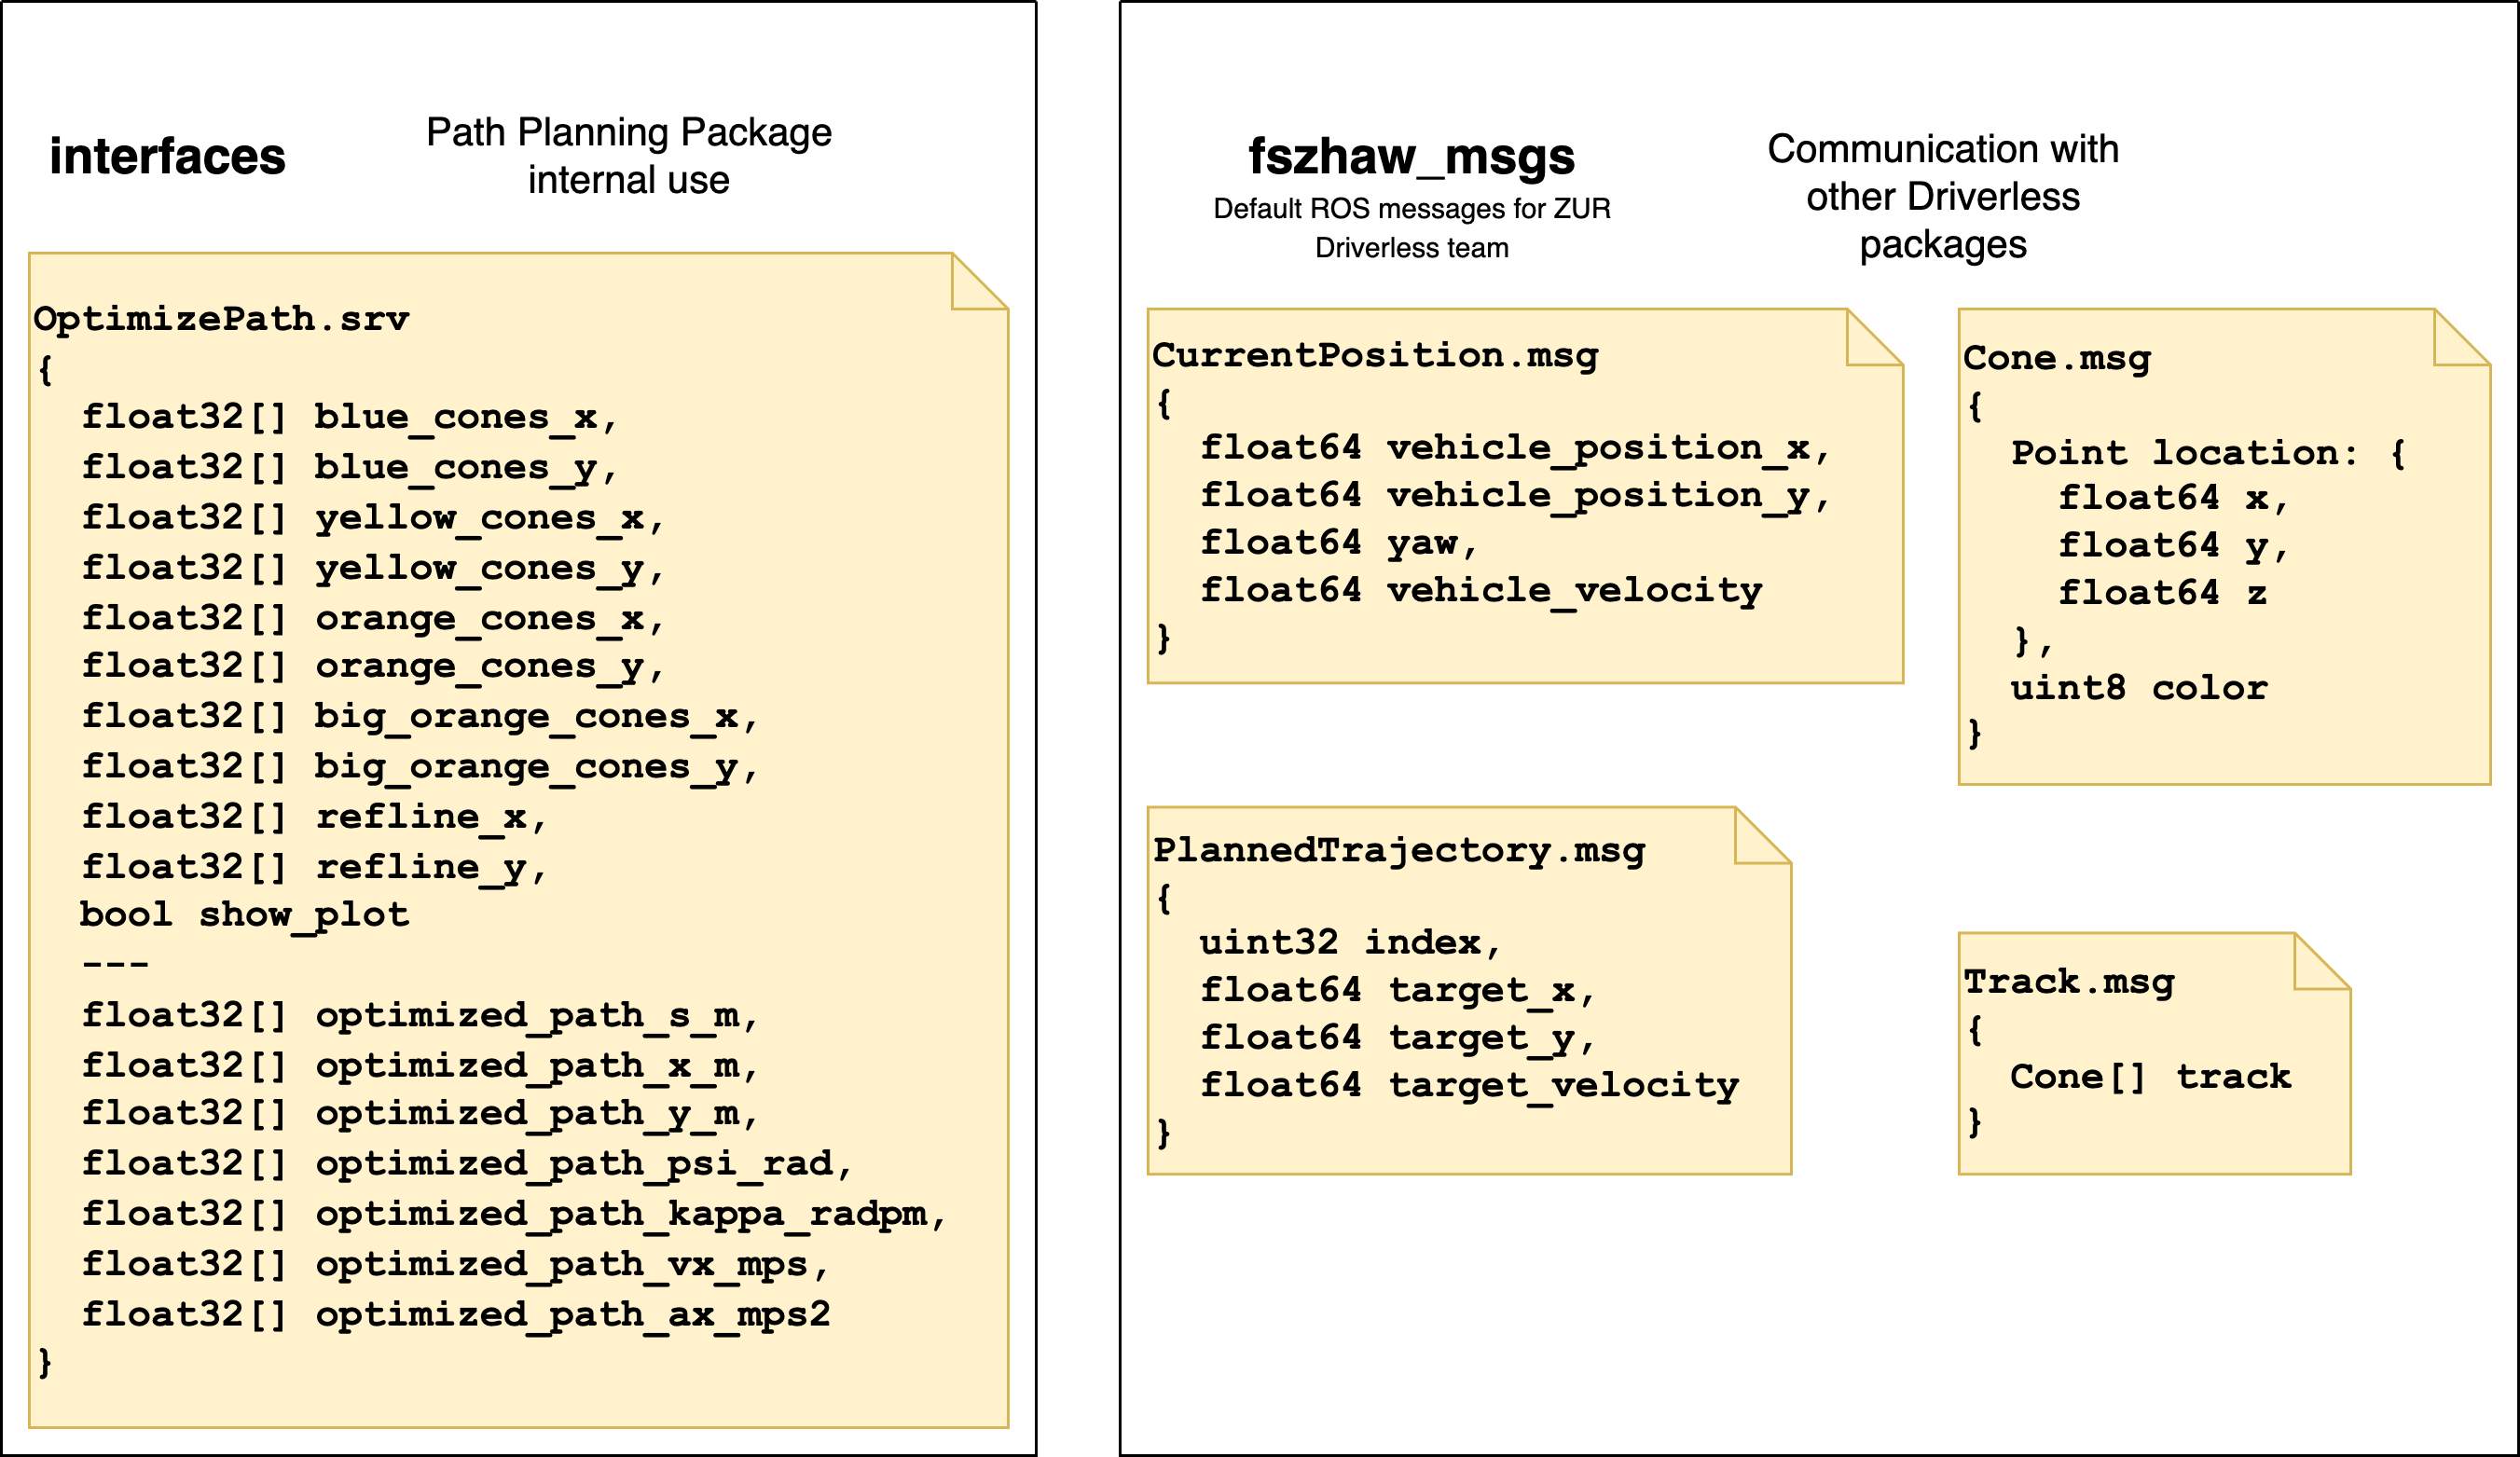
\includegraphics[width=\columnwidth]{Path_Planning_ROS_Messages.png}
    \caption{While the custom \acrshort{ros} messages in the 'interfaces' package are only used in the path planning package internally, the messages in the 'fszhaw\_msgs' package are used to communicate with the other packages in the autonomous system.}
    \label{fig:Path Planning ROS Messages}
\end{figure}
While the 'interfaces' package contains path planning internal ROS messages, the 'fszhaw\_msgs' package contains the messages for communication with the rest of the system. The 'OptimizePath.srv' message is used by the 'optimize\_path' service for the communication between the Path Planner and the Optimization Service, as seen in figure \ref{fig:Path Planning ROS Architecture}. From the 'fszhaw\_msgs' package, following messages are used in the Path Planning component: 'Cone.msg' for the 'cone' topic, 'CurrentPosition.msg' for the 'current\_position' topic, 'PlannedTrajectory.msg' for the 'planned\_trajectory' topic, and 'Track.msg' for the 'testing\_only/track' topic used in combination with the Simulation Tool.

\subsection{Path Planner Node} \label{sec:Path Planner Node}
As seen in the component architecture of the Path Planning package in figure \ref{fig:Path Planning ROS Architecture}, the Path Planner node is the central processor of the whole package.
While receiving the detected cones and current position by the subscribers, the 'Start Finish Detector' can discern if the vehicle has reached the start of the track again. If not, the planner will calculate the planned path using the Exploration Algorithm and output it via the publisher. If a full lap has been completed, the planner will send a request for optimization to the 'Optimization Service'. After receiving the optimized path, it will send that via the publisher instead of the path calculated by the Exploration Algorithm. An overview of the Path Planner Node can be seen in figure \ref{fig:Path Planning Path Planner Node}.
\begin{figure}[H]
    \centering
    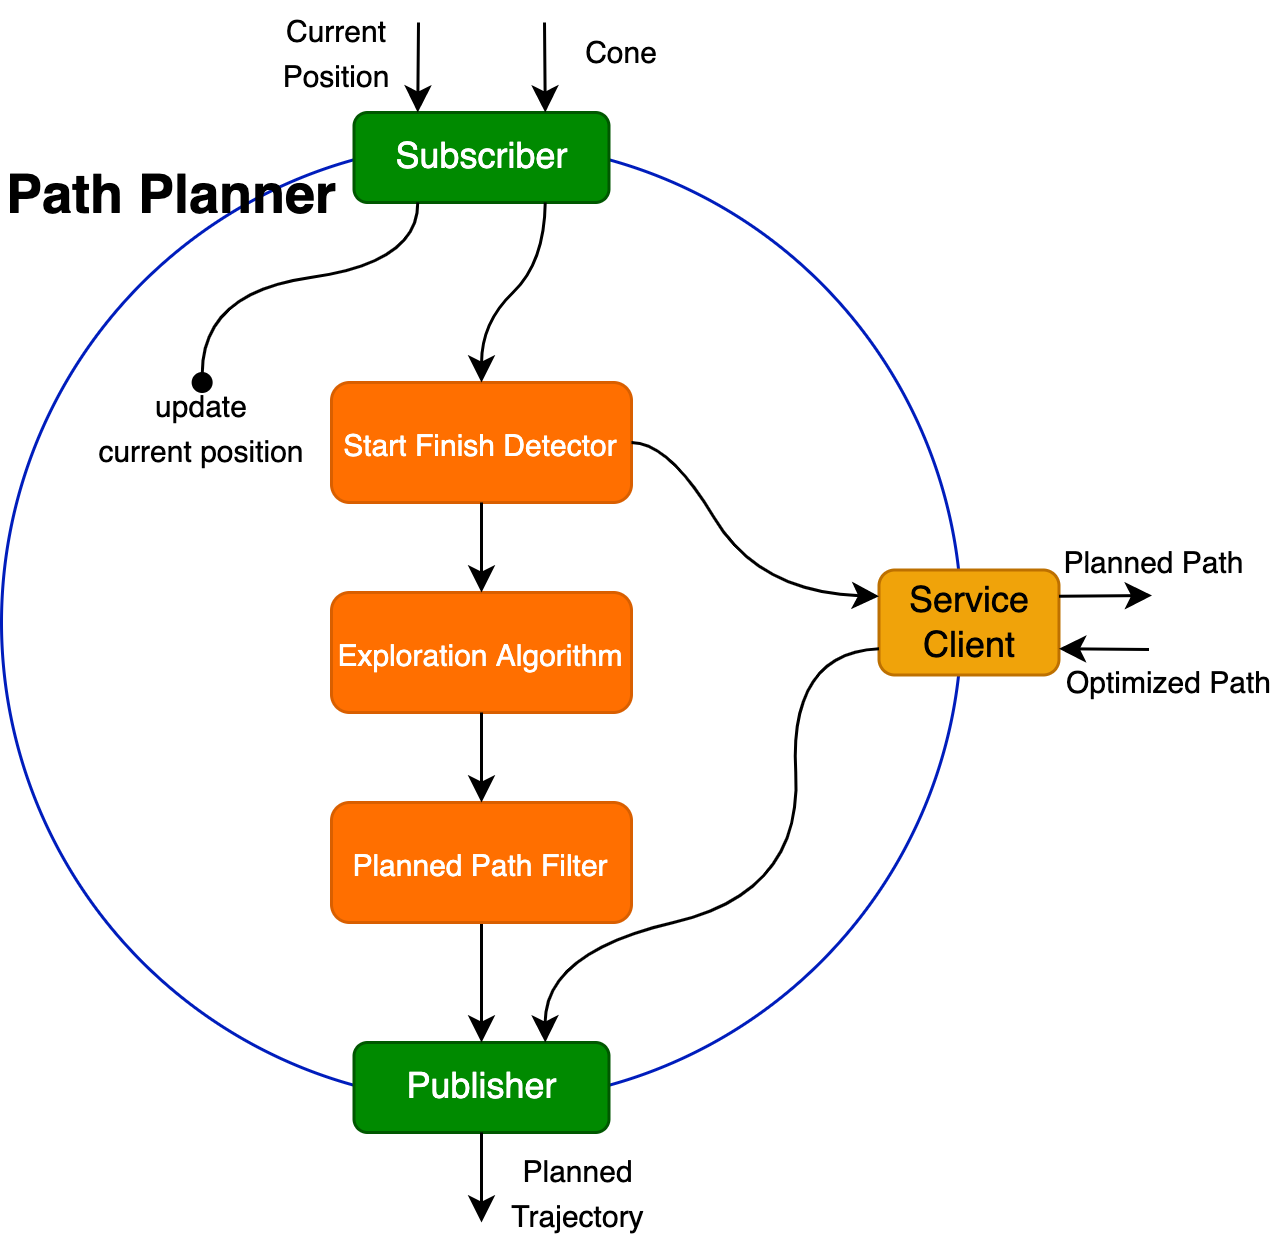
\includegraphics[width=8cm]{Path_Planning_Path_Planner.png}
    \caption{The Path Planner Node is made up of several components, a component for detecting the start of the track, the Exploration algorithm itself and the \acrshort{ros} subscriber, publisher and service client.}
    \label{fig:Path Planning Path Planner Node}
\end{figure}

\subsubsection{Start Finish Detector} \label{sec:Start Finish Detector}
The 'Start Finish Detector' is responsible for realizing when the start or rather the end of the track has been reached. There are two different ways the detector detects such a finish: By comparing its current position with the initial starting position or by detecting several big orange cones, which mark the starting line of a lap.

For events where the tracks are fully enclosed circuits, the end of a lap can be detected by just comparing the car's current position with the initial starting position at the beginning of the event. As illustrated in figure \ref{fig:Path Planner Start Finish Detector 1}.
\begin{figure}[H]
    \centering
    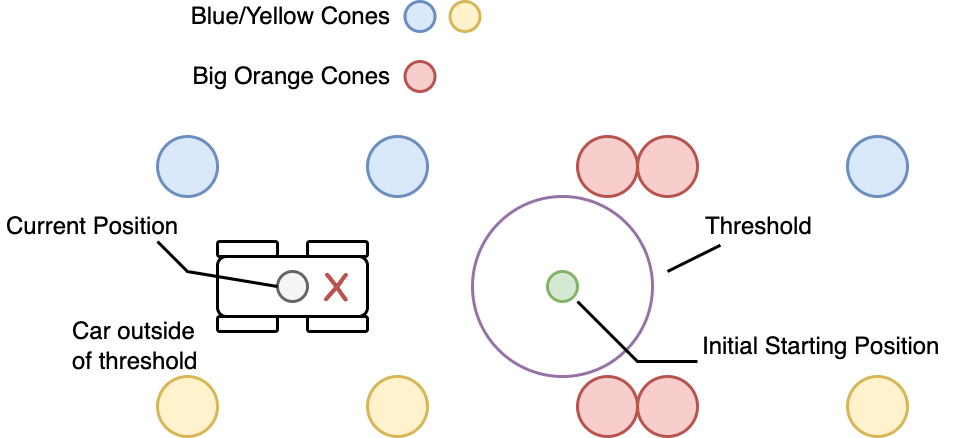
\includegraphics[width=\columnwidth]{Path_Planner_Start_Finish_Detector_1.png}
    \caption{Situation while the car hasn't reached the threshold of the initial starting position.}
    \label{fig:Path Planner Start Finish Detector 1}
\end{figure}
The class will detect the completion of the lap as soon as the car reaches the threshold surrounding the initial starting position.
\begin{figure}[H]
    \centering
    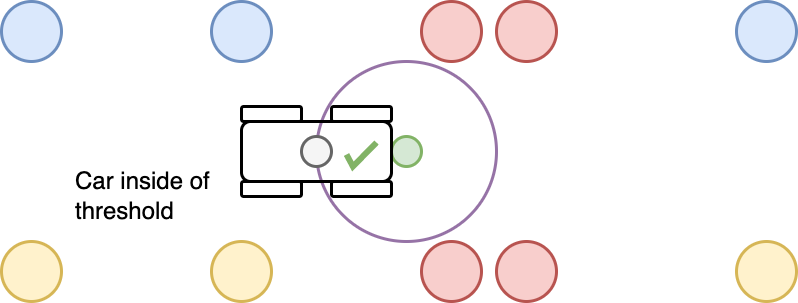
\includegraphics[width=\columnwidth]{Path_Planner_Start_Finish_Detector_2.png}
    \caption{Situation if the car reaches the threshold surrounding the initial starting position.}
    \label{fig:Path Planner Start Finish Detector 2}
\end{figure}

For events where the initial starting position isn't also the start respectively the end of a track, as with the Acceleration or Skidpad event, the starting line needs to be detected by encountering big orange cones, which mark the end of a track. These detected cones need to be close enough to be counted as a valid start/finish cone, or else they will be ignored, as seen in figure \ref{fig:Path Planner Start Finish Detector 3}.
\begin{figure}[H]
    \centering
    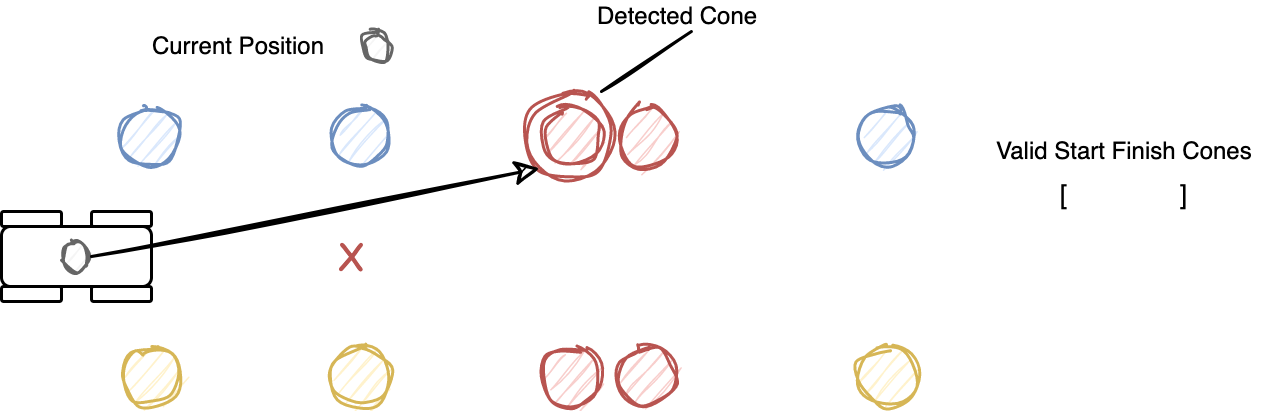
\includegraphics[width=\columnwidth]{Path_Planner_Start_Finish_Detector_3.png}
    \caption{The cone will be disregarded, as it is outside the threshold distance.}
    \label{fig:Path Planner Start Finish Detector 3}
\end{figure}
As soon as a big orange cone gets detected inside the threshold, it will be added as a valid start/finish cone, as illustrated in figure
\begin{figure}[H]
    \centering
    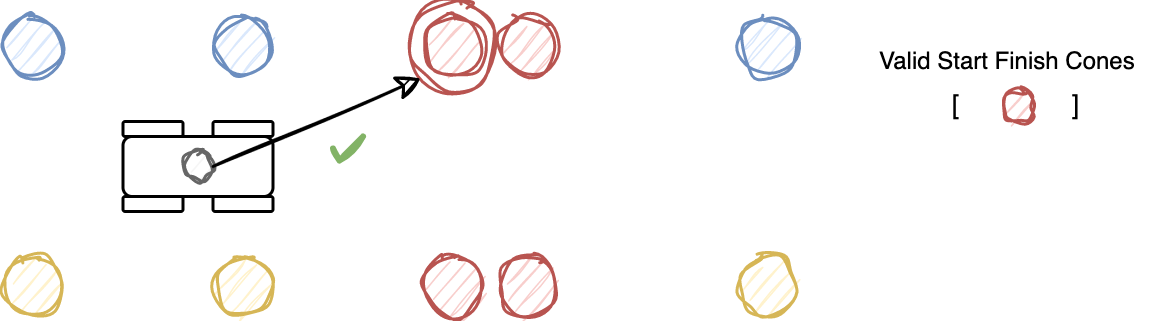
\includegraphics[width=\columnwidth]{Path_Planner_Start_Finish_Detector_4.png}
    \caption{The cone will be added as a valid start/finish cone, as its distance is inside the threshold.}
    \label{fig:Path Planner Start Finish Detector 4}
\end{figure}
After enough valid start/finish cones get added, e.g. two cones, will the detector check the distances between the added cones, to see if they are really in the same area. If so, will the class successfully detect the completion of the track. As illustrated in figure \ref{fig:Path Planner Start Finish Detector 5}.
\begin{figure}[H]
    \centering
    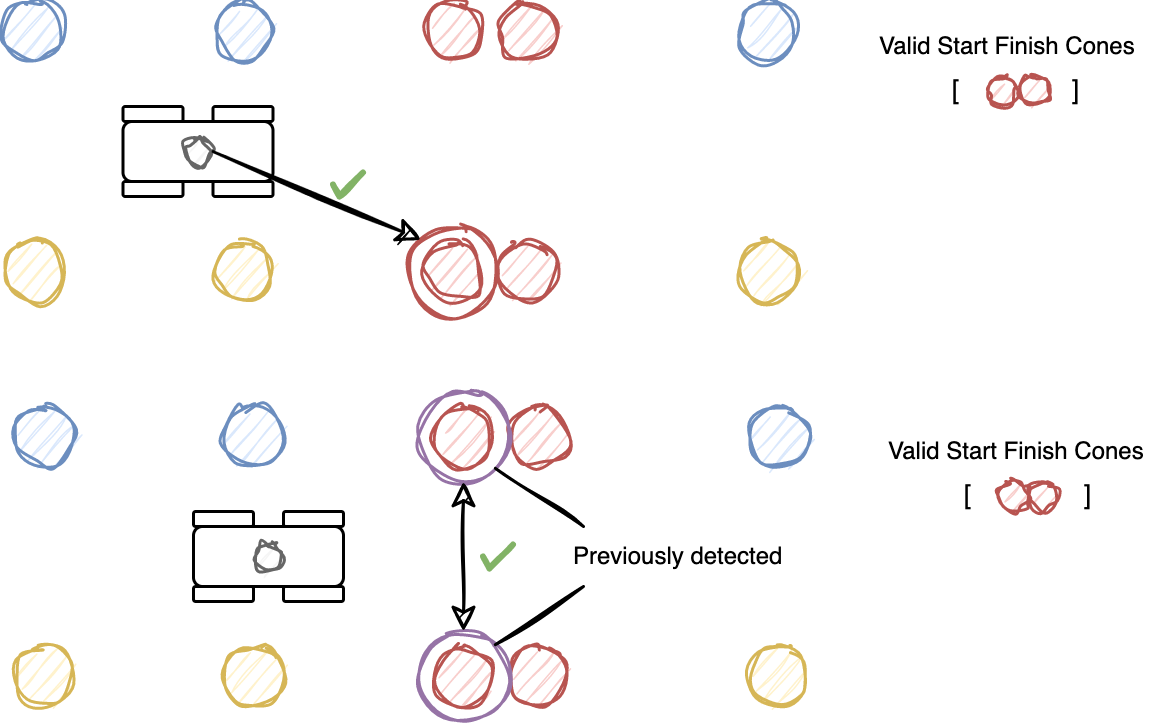
\includegraphics[width=\columnwidth]{Path_Planner_Start_Finish_Detector_5.png}
    \caption{Two valid start/finish cones get added and the completion of the track is successfully detected.}
    \label{fig:Path Planner Start Finish Detector 5}
\end{figure}

\subsubsection{Exploration Algorithm} \label{sec:Exploration Algorithm}
The exploration algorithm implementation is found in the python file: ``src/path\_planning/path\_planning/algorithm/exploration/exploration.py''. The algorithm uses several steps to get the middle line out of the cones position and car position on the track. Figure \ref{fig:Algorithm Exploration Figure A} and \ref{fig:Algorithm Exploration Figure B} are illustrating the different steps of the algorithm. Starting of with the steps (a) to (e) from figure \ref{fig:Algorithm Exploration Figure A}. The algorithm starts when more than 2 cones have been received from the ``cone\_publisher''. Step (a) shows 5 cones that have been received so far, the current position of the car and the next cone. After having enough cones the algorithm calculates the distance from the car to the newly received cone and evaluates the distance based on a threshold which is defined in a track configuration file. If the distance is in the threshold then new distances are calculated from the new cone to the previously received ones as shown in step (c). This distance has a different threshold and evaluates if the previously received cones are good for triangulation. Then the triangulation between the cones in the threshold and the new cone are calculated. This is shown in step (d). After the calculation of the triangles simplices are evaluated between the cones (e). These simplices or triangles consist of several edges.

\begin{figure}[H]
    \centering
    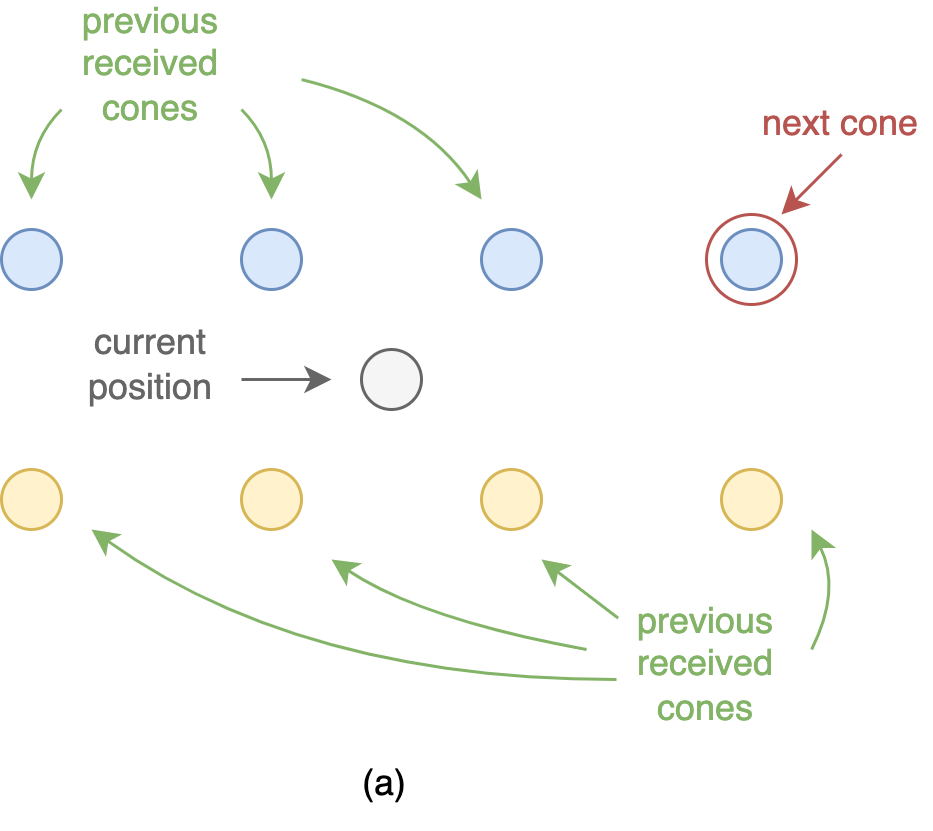
\includegraphics[width=5.5cm]{Algorithm_Exploration_Figure_A.png}
    \caption{The exploration algorithm covers the steps to find a middle line on the track. The first part of the algorithm describes the steps to find suitable cones for the triangulation algorithm (steps a to e).}
    \label{fig:Algorithm Exploration Figure A}
\end{figure}

Figure \ref{fig:Algorithm Exploration Figure B} shows the second part of the algorithm. It starts of based on the information of the edges between the new cones and cones in the given threshold. Step (f) shows how useful edges are validated. Edges which do not have the same tag meaning the same cone color on each side are not usable. The second criterion is that the edge can not be too long which becomes especially relevant in a curve on the track. This process of evaluation is repeated for every simplices (g). The next step (h) is to build a path. Since the path is not smooth an interpolation algorithm is used to straighten the path (i). After that the densify algorithm helps to have a path with more coordinates which is preciser (j). This path will then be published, and the optimization algorithm can use the generated points.

\begin{figure}[H]
    \centering
    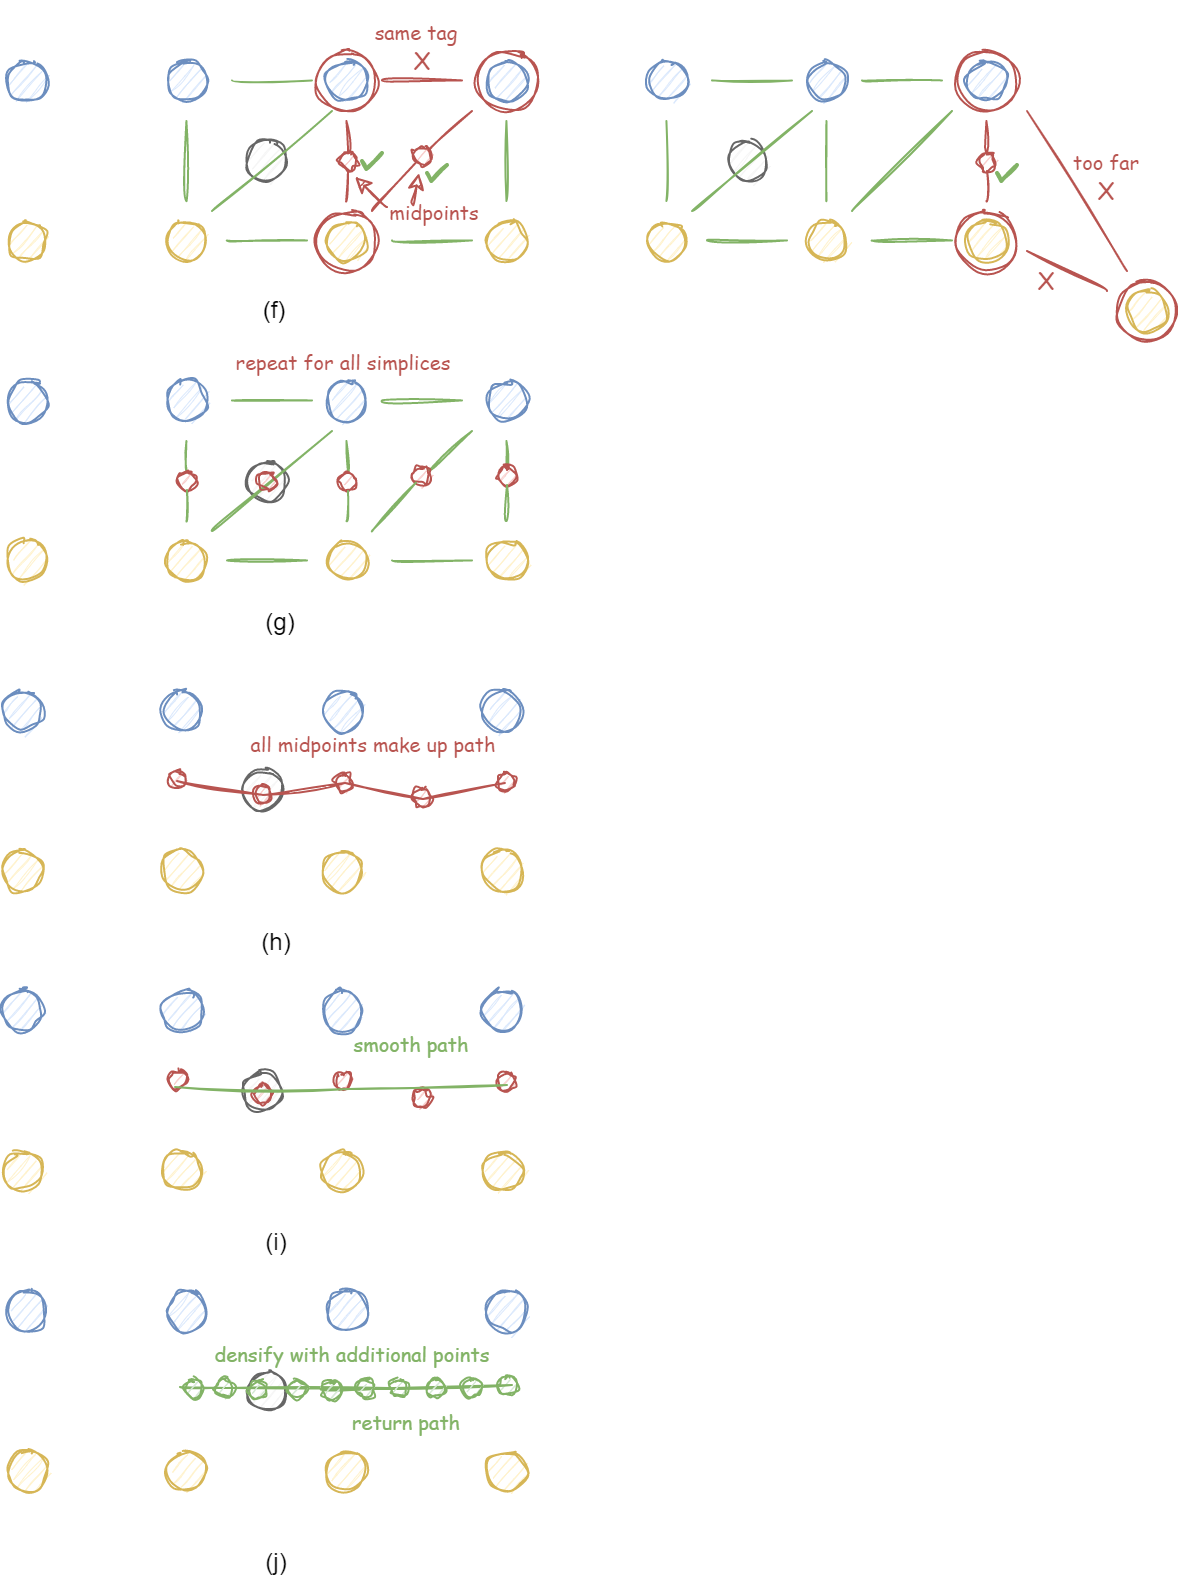
\includegraphics[width=10cm]{Algorithm_Exploration_Figure_B.png}
    \caption{The second part of the exploration algorithm covers criteria of suitable edges in a simplex, smoothening the path and denisifying the smoothed path.}
    \label{fig:Algorithm Exploration Figure B}
\end{figure}

Figure \ref{fig:Algorithm Exploration Pseudocode} shows the pseudocode of the exploration algorithm. Starting of with the distance from the current position of the car to the new cone the program checks if the distance is in the threshold. After that a list is created with all the past cones that are in a valid distance to the new cone. If the list is in the threshold of 3 or more cones than the triangulation is calculated. Further explanation is found in section \ref{sec:Motion Planning} under ``Combinatorial Motion Planning''. After the calculation of the simplices the edges were compared with each other so that no edges of the same ends are in the variable called ``edges''. After the comparison another loop is done to look if the cones on each edge do not have the same tag meaning the same color and are in a threshold. Each valid edge will be added to the ``pathOfMiddlepoints'' array. After the program knows the potential middle points a path smoothening algorithm is applied followed with a densify algorithm to add more middle points. The final result meaning the middle line as well as the track border is given to the optimization algorithm.

\begin{figure}[H]
    \centering
    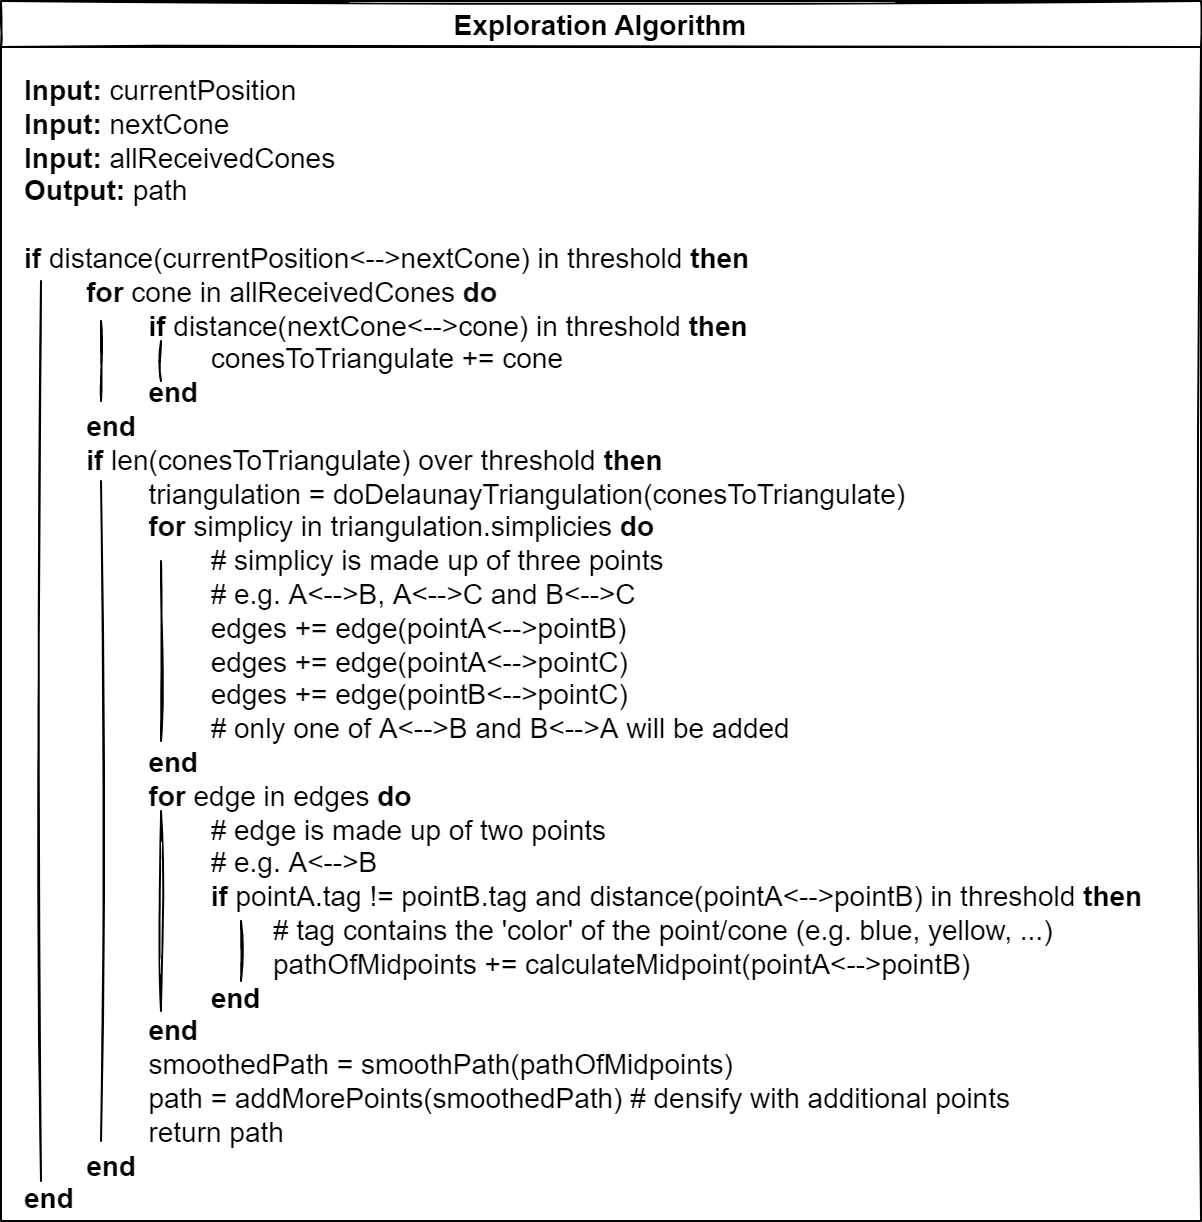
\includegraphics[width=10cm]{Algorithm_Exploration_Pseudocode.png}
    \caption{The exploration algorithm can be presented in a pseudocode program as well.}
    \label{fig:Algorithm Exploration Pseudocode}
\end{figure}

\subsubsection{Planned Path Filter} \label{sec:Planned Path Filter}
\lipsum[1]

\subsection{Optimization Service Node} \label{sec:Optimization Service Node}
The Optimization Service Node is responsible for receiving the request for optimization by the Path Planner Node, preparing the input for optimization, optimizing the path, and then sending it back to the planner for further processing and publishing.

The node is made up of two main components, the 'Optimization Input Transformer' and the 'Optimization Algorithm' itself. The node will receive all previously detected cones and a reference line of the driven track by the planner, e.g. the middle line. In this case, the reference line will be the calculated path by the 'Exploration Algorithm'. Because the 'Optimization Algorithm' expects a single reference line with its distances to the track's border as an input, a transformation of the received input is first needed, before it can be optimized by the algorithm. With the data from all the received cones and reference line, the 'Optimization Input Transformer' is able to map the input to a single list of reference points and the distances from each point to the track's border. The transformer will be explained further in section \ref{sec:Optimization Input Transformer}. With that list, the 'Optimization Algorithm' can optimize the path with regard to one of several objectives, e.g. the shortest path or minimum curvature. The algorithm will be explained in more detail in section \ref{sec:Optimization Algorithm}. The optimized path will then be sent back to the planner via the  \acrshort{ros} service.
\begin{figure}[H]
    \centering
    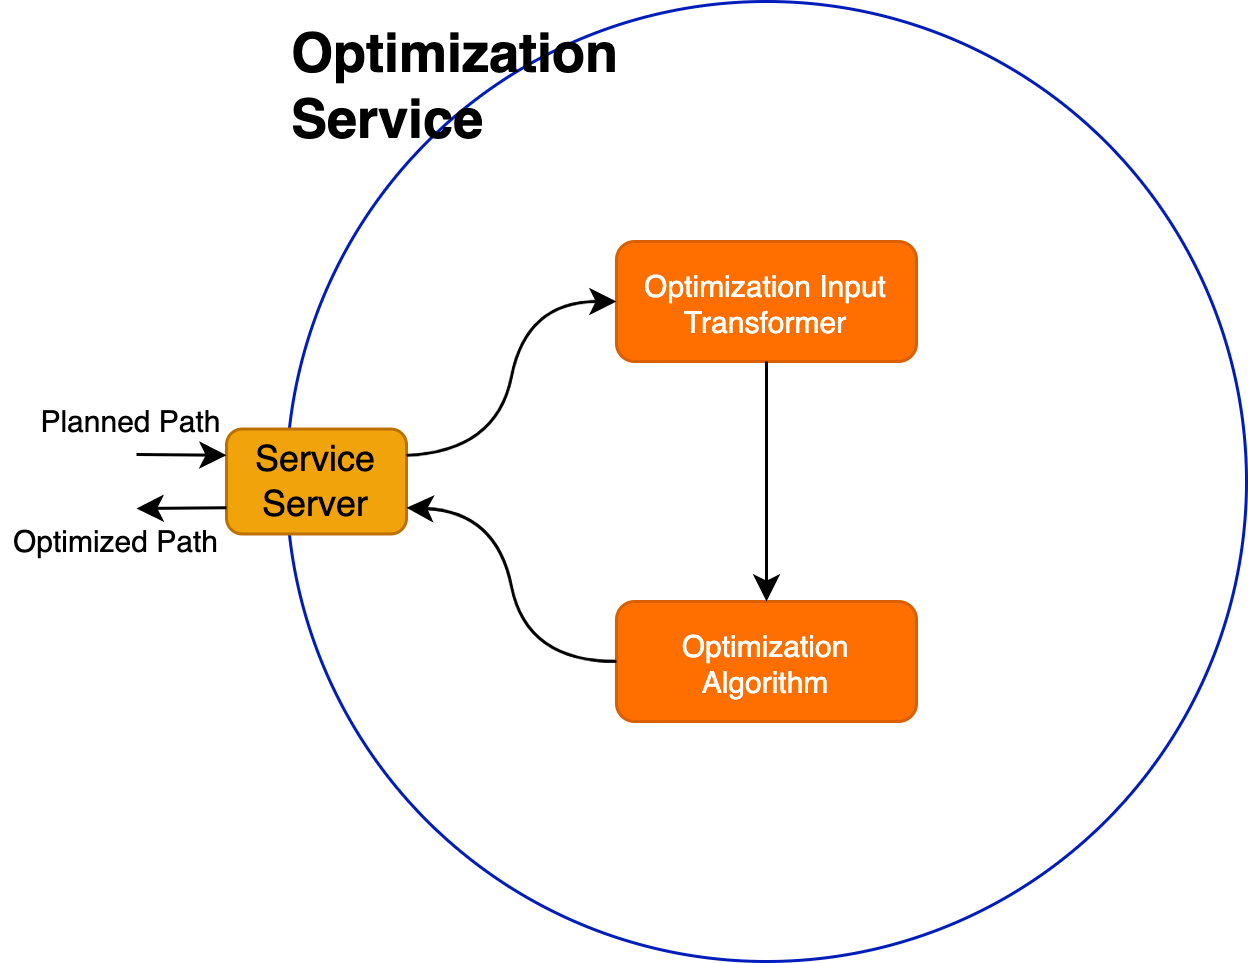
\includegraphics[width=8cm]{Path_Planning_Optimization_Service.png}
    \caption{The Optimization Service Node is made up of two main components, a component for preparing the received input for optimization and the algorithm to optimize the path itself.}
    \label{fig:Path Planning Optimization Service Node}
\end{figure}

\subsubsection{Optimization Input Transformer} \label{sec:Optimization Input Transformer}
As mentioned before in section \ref{sec:Optimization Service Node}, all previously detected cones (blue, yellow, orange and big orange cones) and a reference line, in this case the calculated path by the Exploration Algorithm, are used as input by the Optimization Input Transformer. As the output, a newly created reference track consisting of reference points and their corresponding distances to the track's limits are received. An illustration can be seen in figure \ref{fig:Optimization Service Input Transformer 1}
\begin{figure}[H]
    \centering
    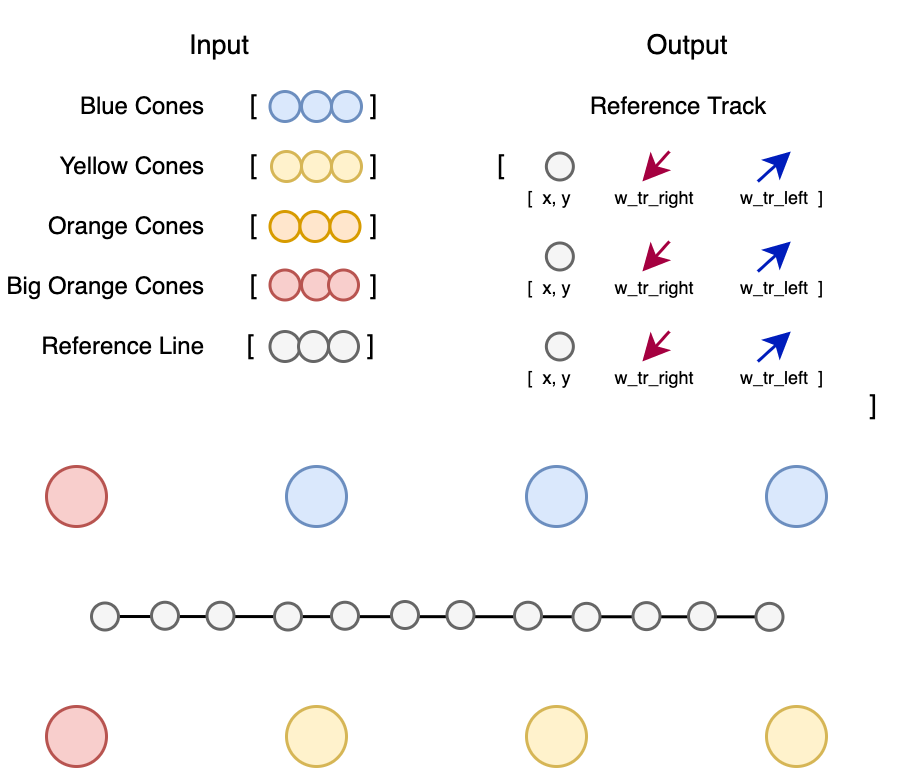
\includegraphics[width=\columnwidth]{Optimization_Service_Input_Transformer_1.png}
    \caption{All previously received cones and a reference line are used as the input, while a reference track containing reference points and their distances to the track limits are received as the output.}
    \label{fig:Optimization Service Input Transformer 1}
\end{figure}
Firstly, for each given yellow or blue cone, the closest point on the reference line will be calculated. For this step, the list with more cones in it will be chosen, the list with all yellow cones would be used if there are more yellow than blue cones. Depending on the position of the orange and big orange cones, they will be classified as a blue or as a yellow cone during this process.
\begin{figure}[H]
    \centering
    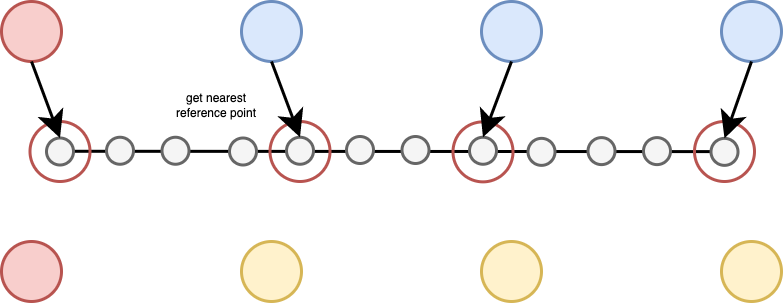
\includegraphics[width=\columnwidth]{Optimization_Service_Input_Transformer_2.png}
    \caption{For each blue or yellow cone, its closest point on the reference line will be determined.}
    \label{fig:Optimization Service Input Transformer 2}
\end{figure}
Secondly, for each reference point, its distance to the track limits are calculated. Because blue cones are always situated on the left side of the track and yellow cones always on the right side, the distance to the left track limit can be determined by computing the distance to its nearest blue cone. For the right track limit, it can be determined by computing the distance to its nearest yellow cone.
\begin{figure}[H]
    \centering
    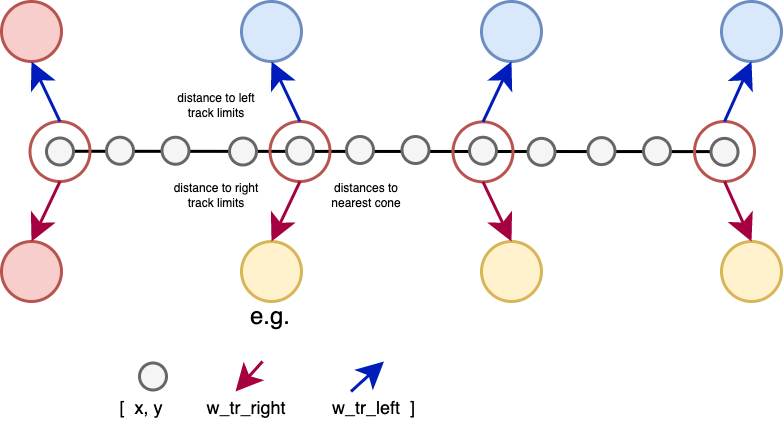
\includegraphics[width=\columnwidth]{Optimization_Service_Input_Transformer_3.png}
    \caption{For each selected reference point, its distance to the left and right track limits will be computed, by just evaluating its distance to the nearest blue cone or yellow cone respectively.}
    \label{fig:Optimization Service Input Transformer 3}
\end{figure}
Lastly, the developed list containing the reference track will then be returned as the output.

\subsubsection{Optimization Algorithm} \label{sec:Optimization Algorithm}
The base code of the implementation was forked from the Institute of Automotive Technology at the \acrlong{tum}.
The repository contains algorithms for determining an optimal racing line. It is possible to choose between several objectives: Shortest Path, Minimum Curvature (with or without iterative call) and Minimum Time (with or without powertrain behaviour consideration). \cite{tumftm_optimization_algoritm}

The racing line from the minimum curvature objective is quite near to a minimum time racing line in corners, but will differ as soon as the car's acceleration limits are not exploited. However, the minimum time optimization requires a lot more parameters and takes more computation time. It was decided to primarily use the Minimum Curvature objective, as the time difference between Minimum Curvature and Minimum Time is too small to justify its use over the other algorithms (see chapter \ref{ch:Results}).

\begin{figure}[H]
    \centering
    \includegraphics[width=\columnwidth]{Algorithm_Optimization_Module.png}
    \caption{The main method ``optimize\_path()'' imports parameters from the vehicle parameter file ``racecar.ini'' and receives its inputs, a reference track, an optional friction map and user configurations, by the client. In the end, an optimal race trajectory line will be outputted.}
    \label{fig:Optimization Algorithm Module Overview}
\end{figure}

\textbf{Overview}

At the centre of the Optimization Algorithm is the main file called ``main\_globaltraj.py''. This file includes the ``optimize\_path()'' function used to optimize the path. It imports various utility functions from the ``helper\_funcs\_glob'' package, it contains functions to import a reference track (``import\_track()''), to prepare the imported reference track for optimization (``prep\_track()'') or to plot resulting figures (``result\_plots()''), just to name a few. As a Python dependency, additional helper functions are imported from the ``trajectory\_planning\_helpers'' repository provided by \acrshort{tumftm}. \cite{tumftm_trajectory_planning_helpers}
These useful helper functions for path and trajectory planning are frequently used in the trajectory planning software stack at \acrshort{tumftm}.
In the end, the most optimal race trajectory line will be outputted by the algorithm.
\begin{figure}[H]
    \centering
    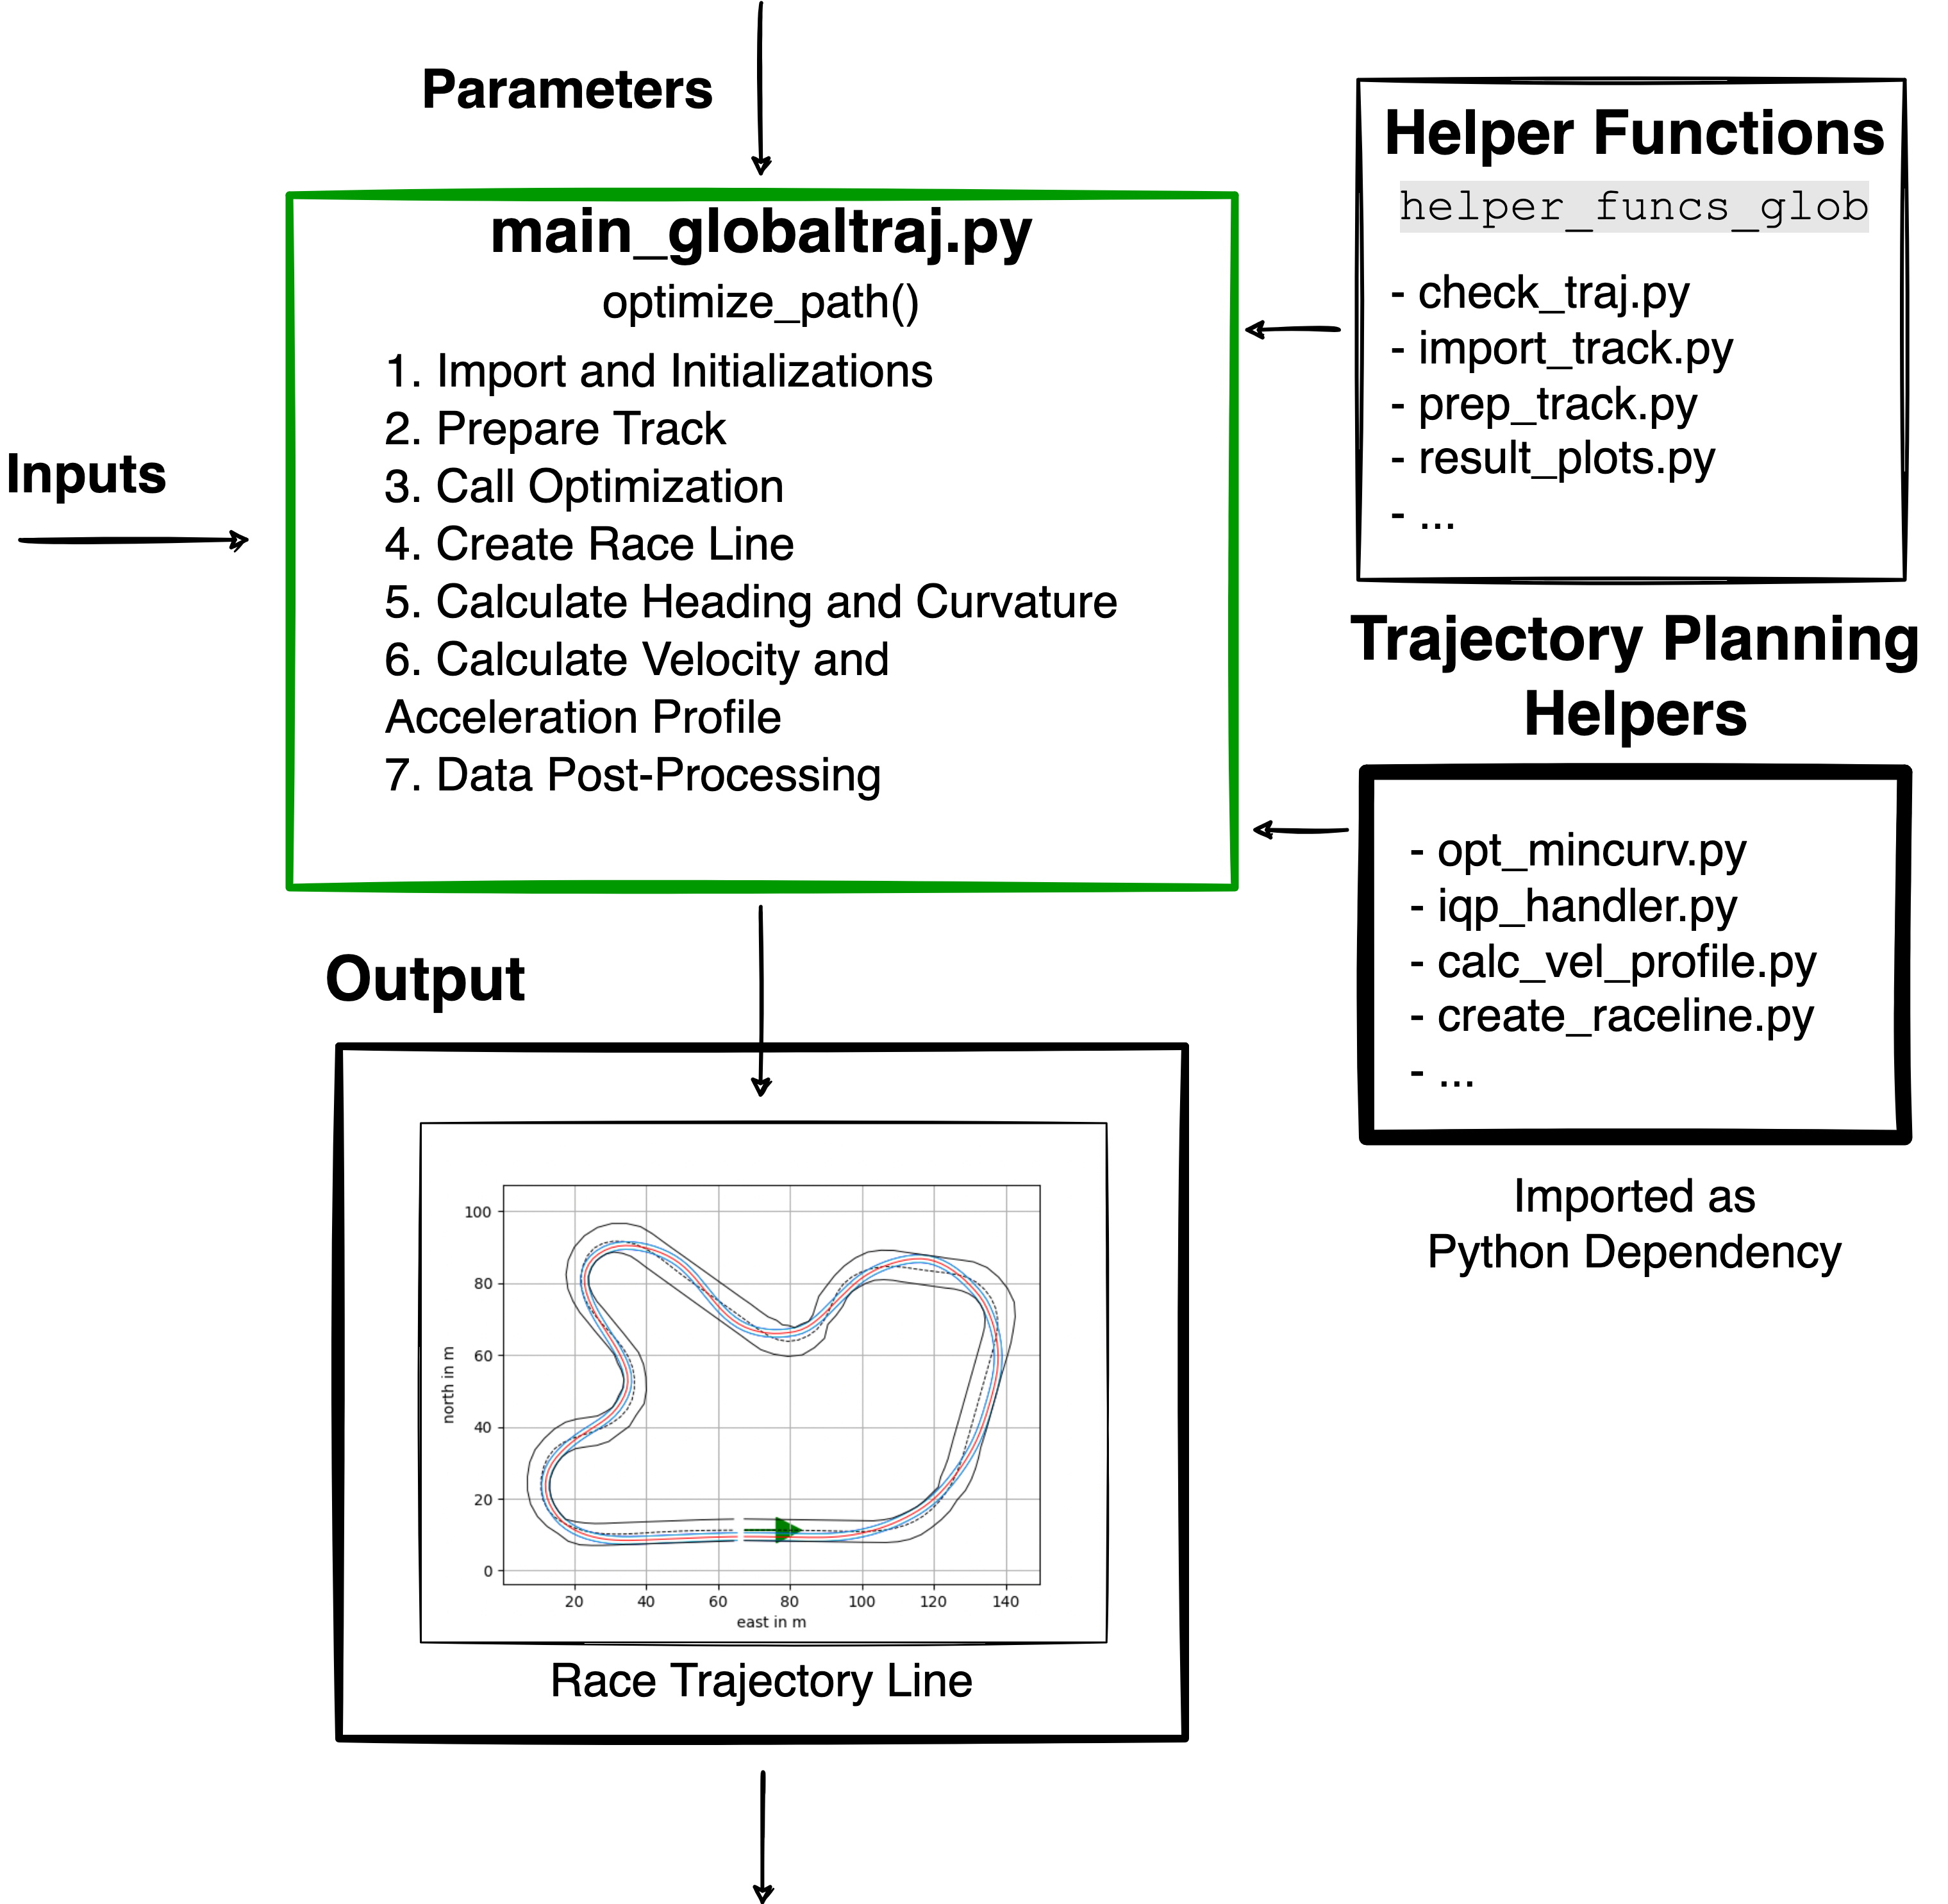
\includegraphics[width=\columnwidth]{Algorithm_Optimization_Module_MainGlobalTraj.png}
    \caption{The main method of the project is located in main\_globaltraj.py and imports important and useful functions from the helper\_funcs\_glob package and the external trajectory\_planning\_helpers repository. The output will be the calculated race trajectory line.}
    \label{fig:Optimization Algorithm Module MainGlobalTraj}
\end{figure}

\textbf{Inputs}

As for its inputs, the main method receives the required reference track and additional user configurations, like the optimization type, minimum track width, number of laps to be driven and more, by the client. A supplementary friction map of the track can also be provided, but is only relevant for Minimum Time solutions. In principle, they can also be considered within the velocity profile calculation of Minimum Curvature solutions. However, this is currently not supported in this implementation. % ADD CITE
\begin{figure}[H]
    \centering
    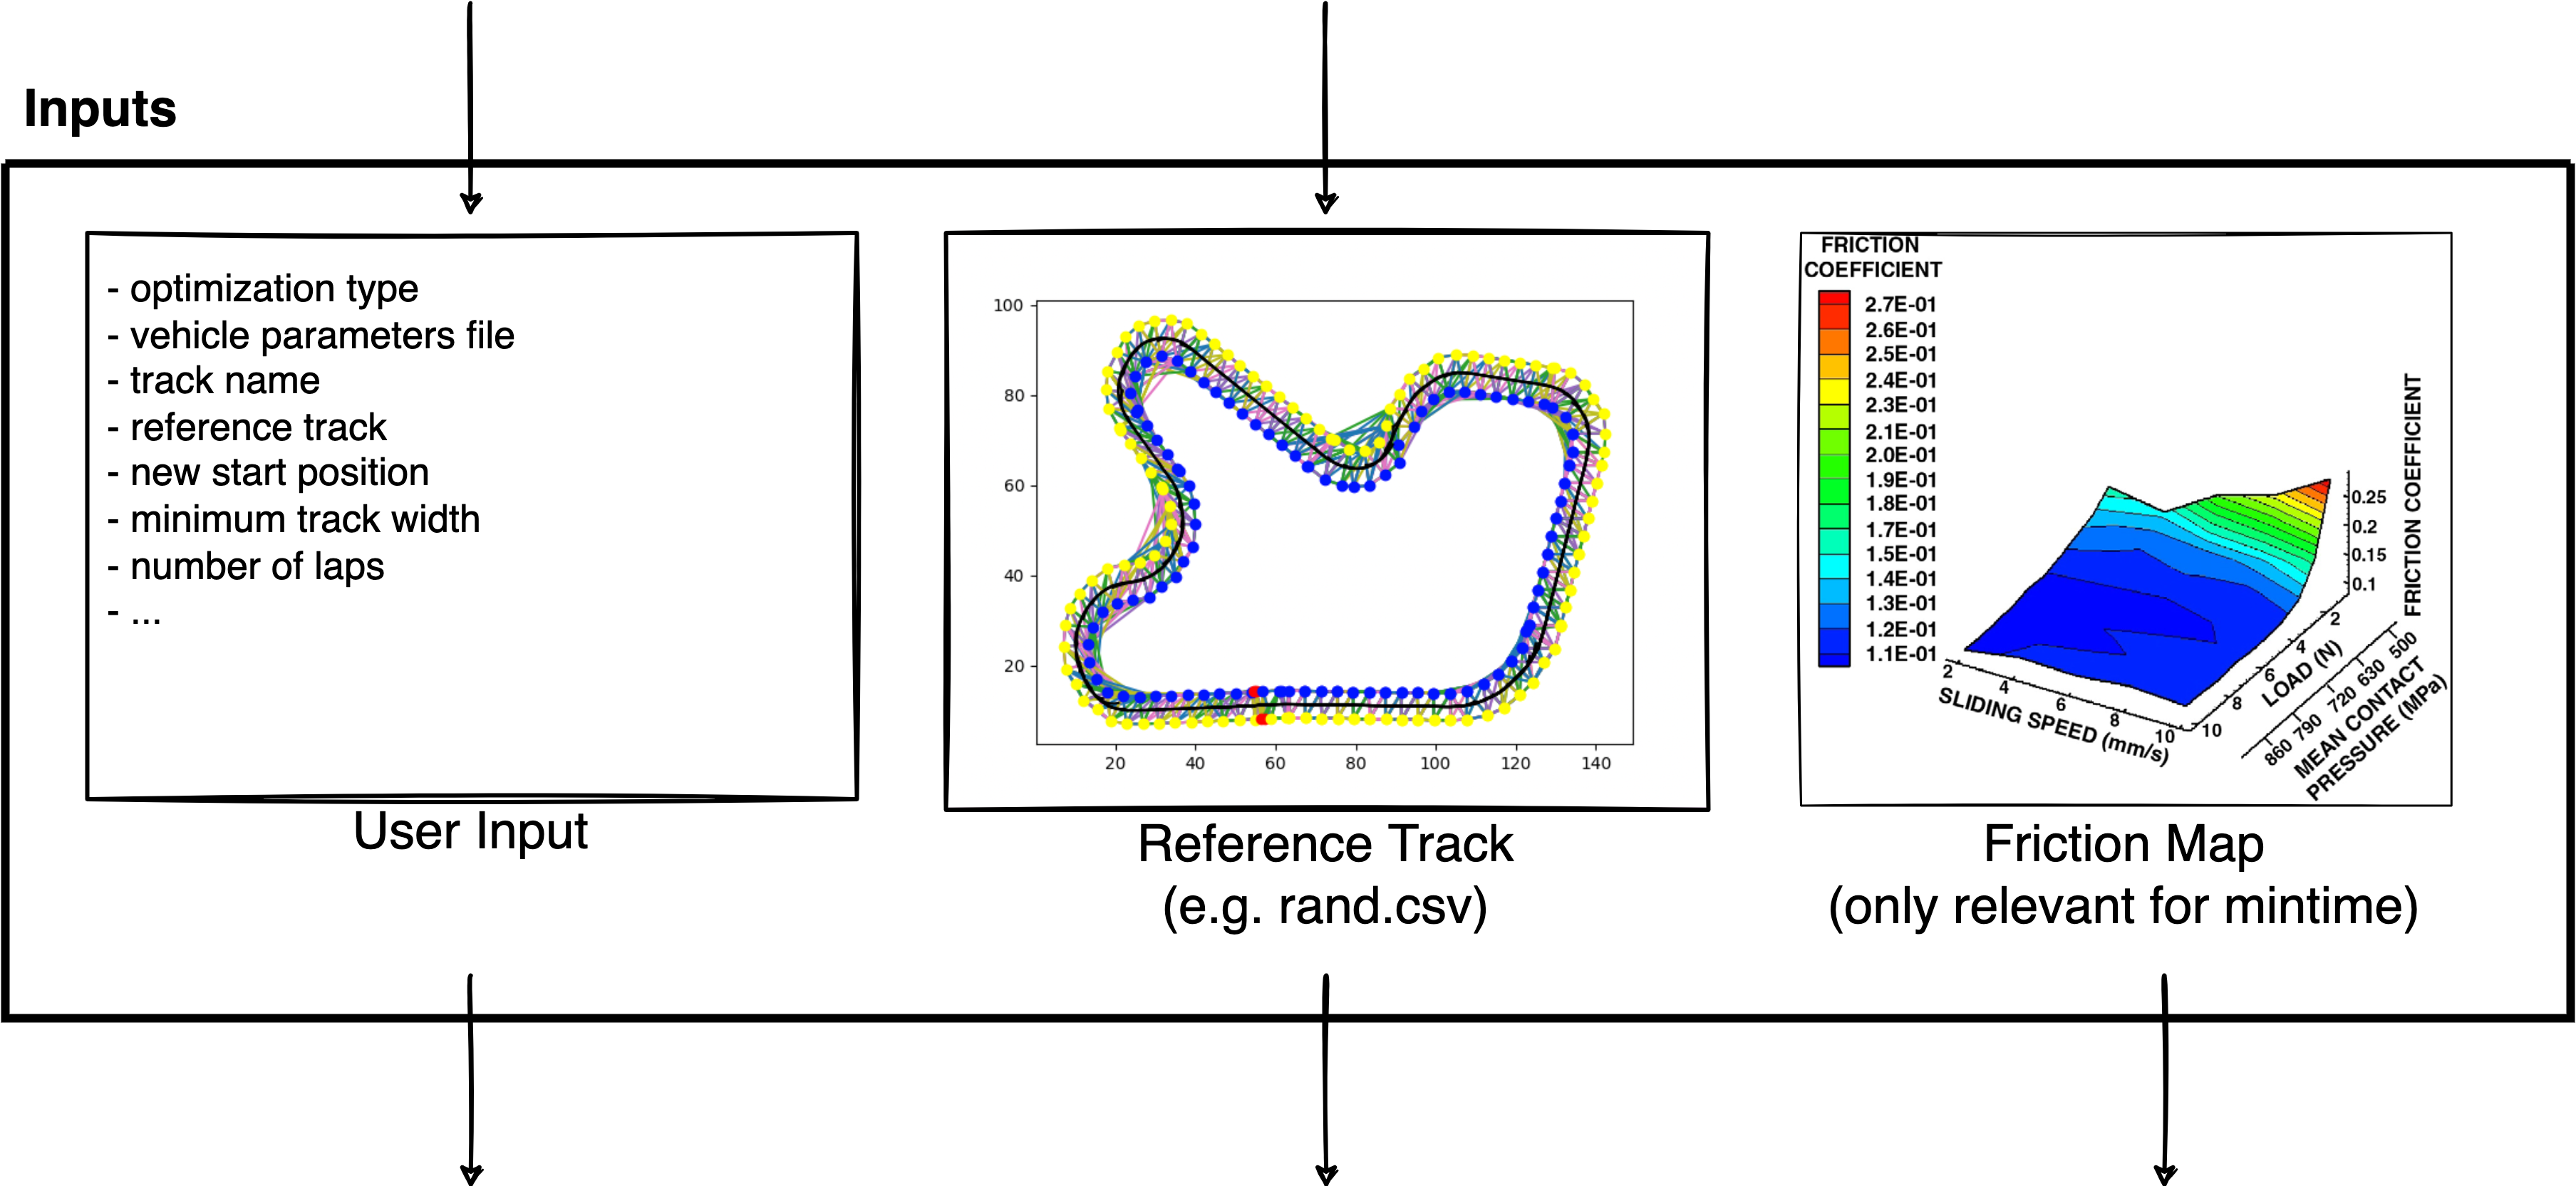
\includegraphics[width=\columnwidth]{Algorithm_Optimization_Module_Inputs.png}
    \caption{The user input and reference track will be received by the client. The friction map is optional and currently only relevant for Minimum Time solutions.}
    \label{fig:Optimization Algorithm Module Inputs}
\end{figure}

Contained in the ``frictionmap'' package of the project, functions related to the creation and handling of friction maps along the racetrack are provided.
The script contained in ``main\_gen\_frictionmap.py'' can be used to create custom friction maps for any racetrack supplied. The explanation behind the friction map generation is out of scope in this thesis, but can be read in ``A Concept for Estimation and Prediction of the Tire-Road Friction Potential for an Autonomous Racecar'' by L. Hermansdorfer, J. Betz and M. Lienkamp. \cite{friction_map_generation}
\begin{figure}[H]
    \centering
    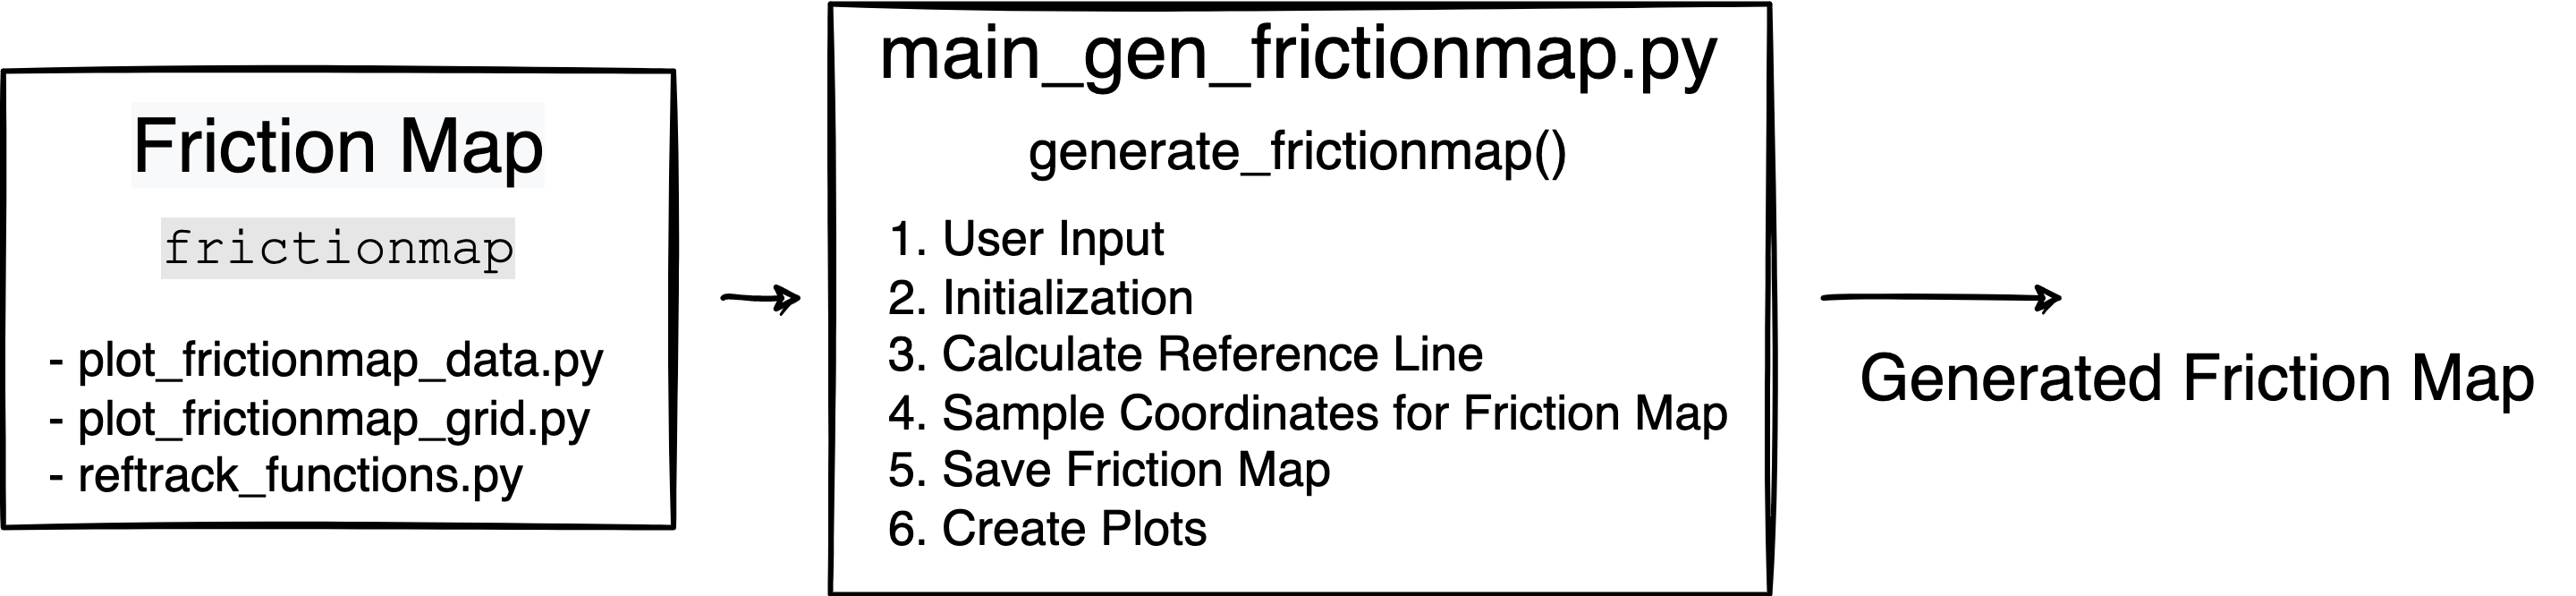
\includegraphics[width=\columnwidth]{Algorithm_Optimization_Module_FrictionMap.png}
    \caption{Overview of the Friction Map package containing functions related to the handling and creation of friction maps.}
    \label{fig:Optimization Algorithm Module Overview}
\end{figure}

\textbf{Parameters}

Parameter-wise, the main method receives everything it needs by the vehicle parameter file called ``racecar.ini''. This file holds general vehicle parameters like the maximum vehicle speed, the length, width and mass of the vehicle, its drag coefficient and its curvature limit. Additionally, the parameter file also holds several calculation options like the step size used for interpolations, smoothing options for spline regression and more.

The vehicle parameter file also sets vehicle dynamics information to be loaded from several files, from a supplementary GGV diagram (``ggv.csv''), also known as the performance envelope, and from a supplementary file called ``ax\_max\_machines.csv'', containing an array with the longitudinal acceleration limits by the electrical motors, as seen in figure \ref{fig:Optimization Algorithm Module Parameters}. If a GG diagram shows the acceleration a car can achieve at a given speed, then a GGV diagram would show the maximum acceleration a car can sustain in any horizontal direction when travelling at any speed. The task of the driver would then be to take the car to the boundaries of its performance envelope at every moment, while the task of the engineers would be to expand the performance envelope of the car by improving on its tires, aerodynamics, powertrain and more.
% ADD CITE
\begin{figure}[H]
    \centering
    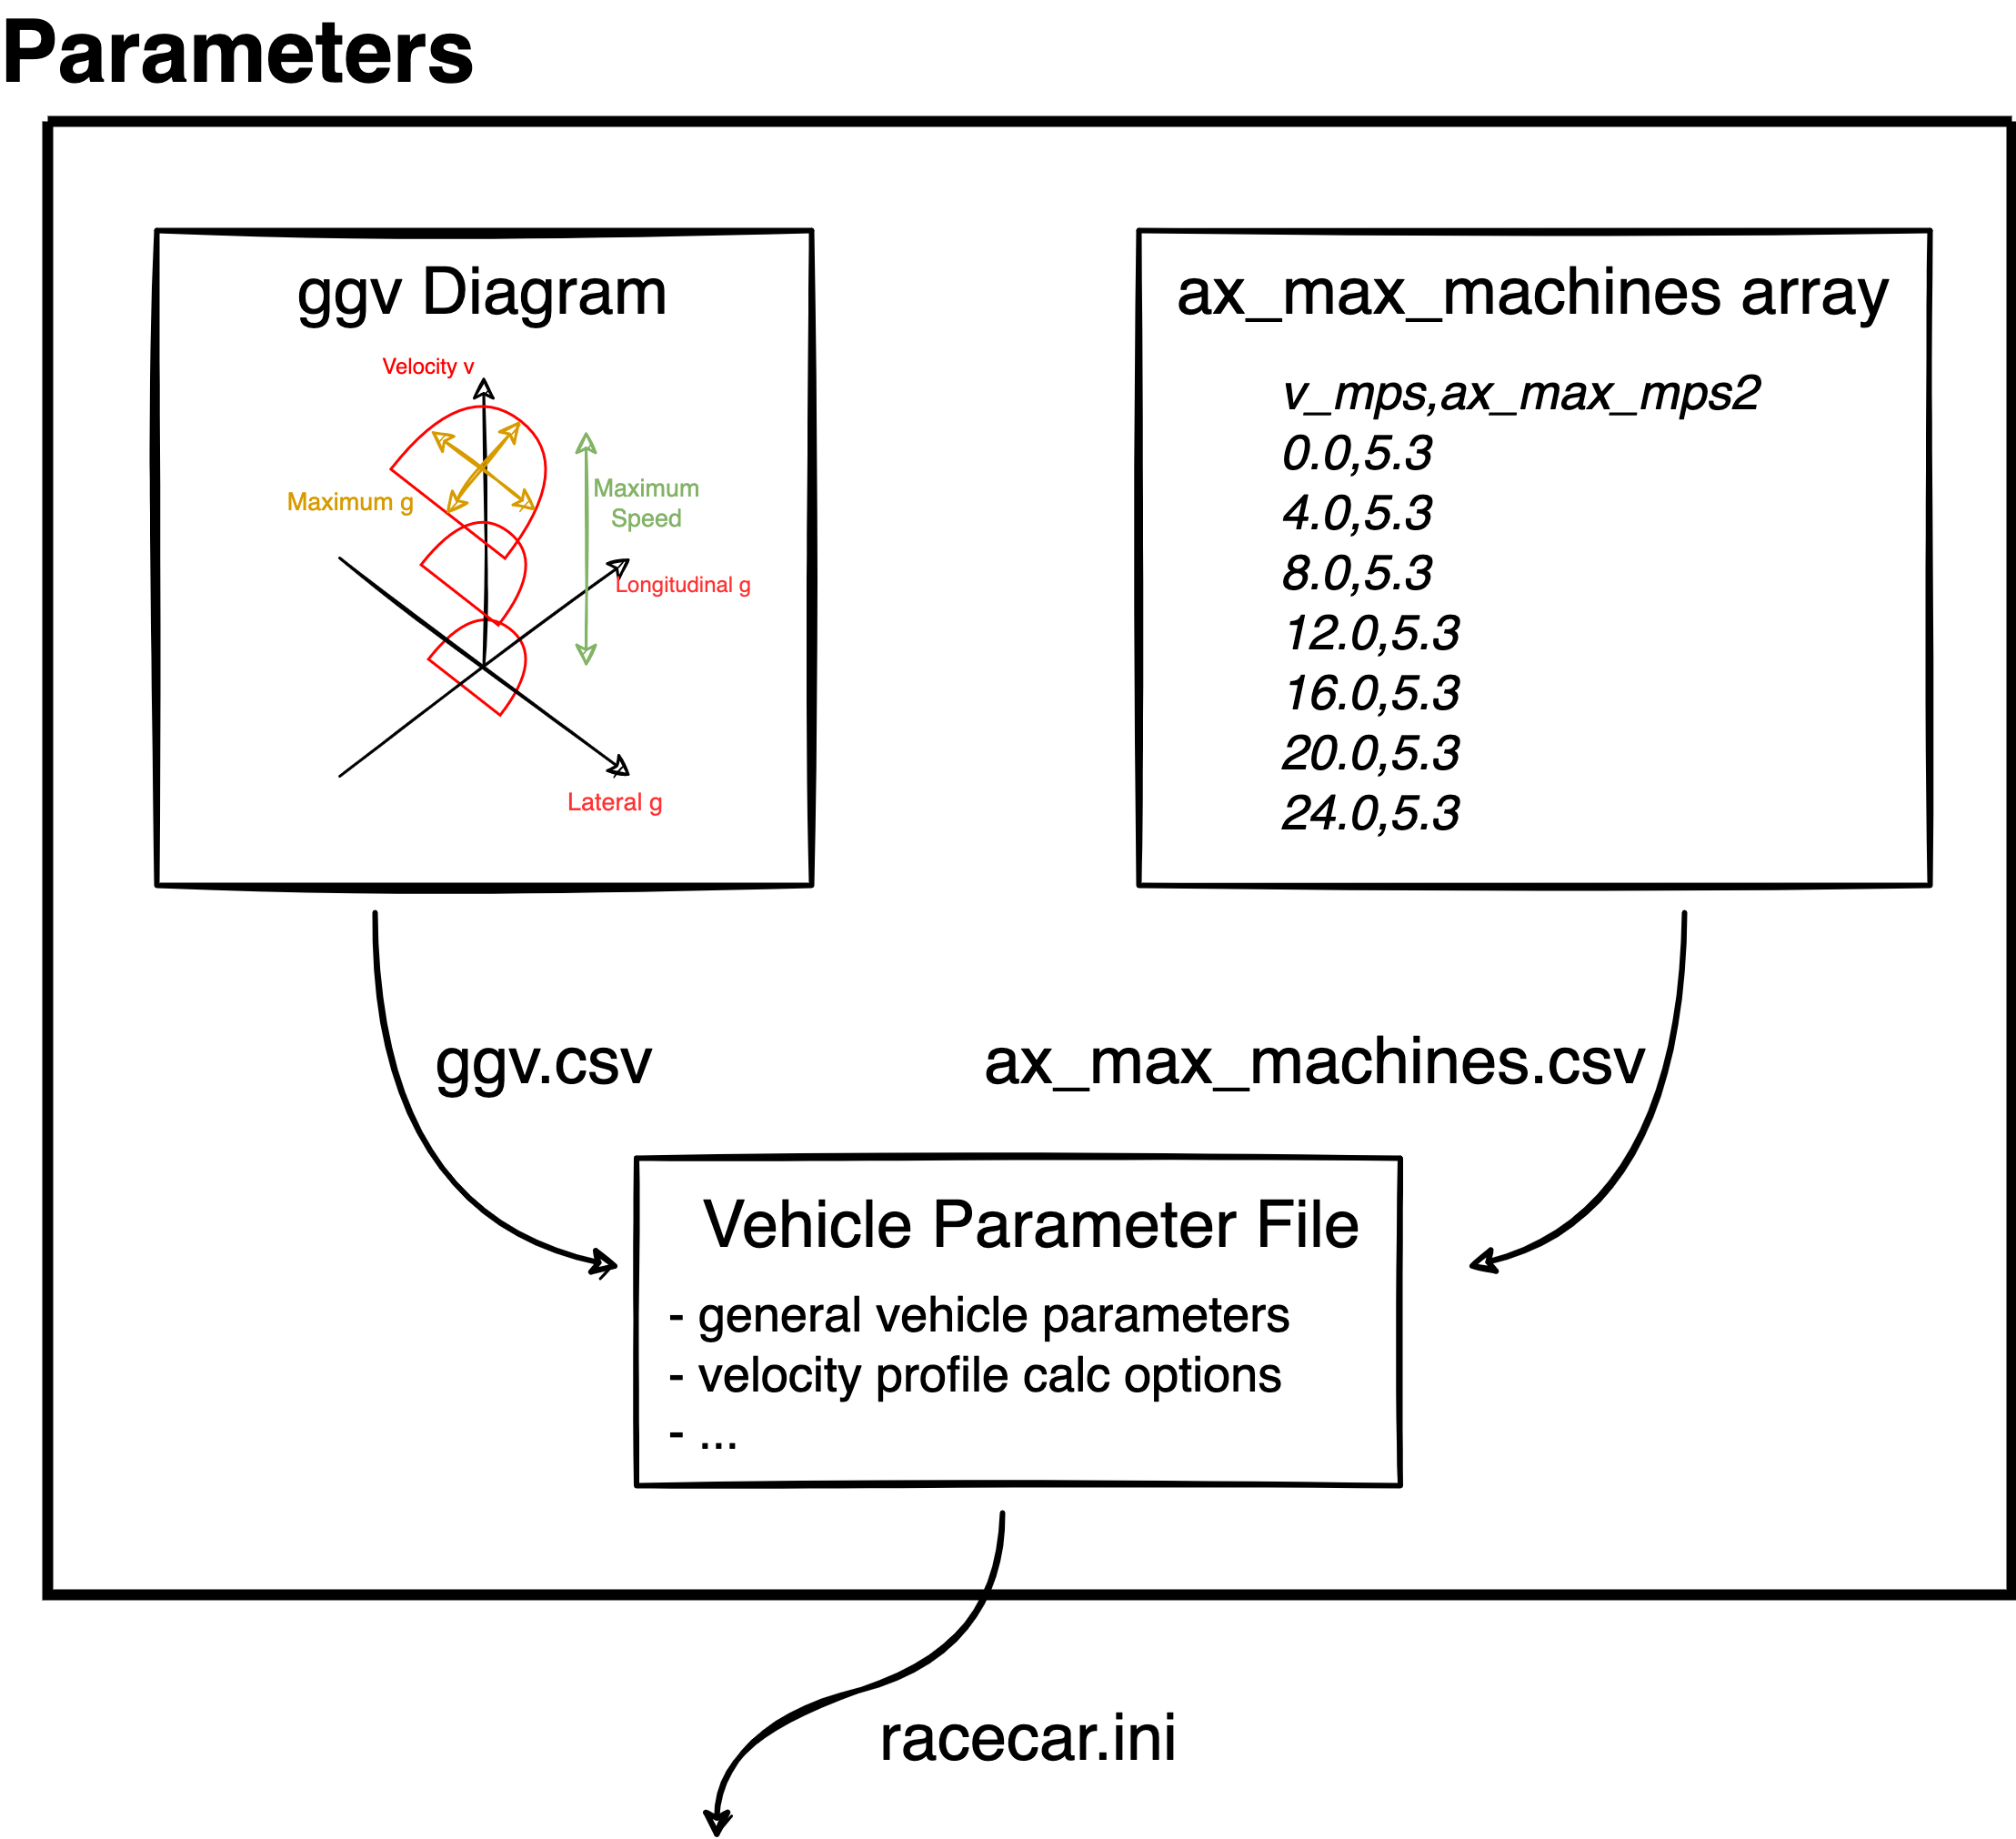
\includegraphics[width=\columnwidth]{Algorithm_Optimization_Module_Parameters.png}
    \caption{The vehicle parameter file, holding general vehicle parameters and several calculation options, receives additional data by the GGV diagram and the ax machines array.}
    \label{fig:Optimization Algorithm Module Parameters}
\end{figure}

\textbf{1. Import and Initializations}

The main method will first load, set and check the input provided by the user. After that, all required paths to the parameter file, output destinations and more will be initialized. And after that, the vehicle dependent parameters can be imported from the ``racecar.ini'' file. The additional vehicle dynamics data will be imported by the ``import\_veh\_dyn\_info()'' helper function. The helper function ``import\_track()'' then imports the track itself, with the input provided by the Optimization Input Transformer.

\textbf{2. Prepare Track}

At the next step, the imported track needs to be prepared for optimization by calling the ``prep\_track()'' utility function.

Firstly, it interpolates the reference track by obtaining a smoothed track on the basis of a spline approximation. Secondly, it calculates the splines by solving for curvature continuous cubic splines between the given points.
\begin{figure}[H]
    \centering
    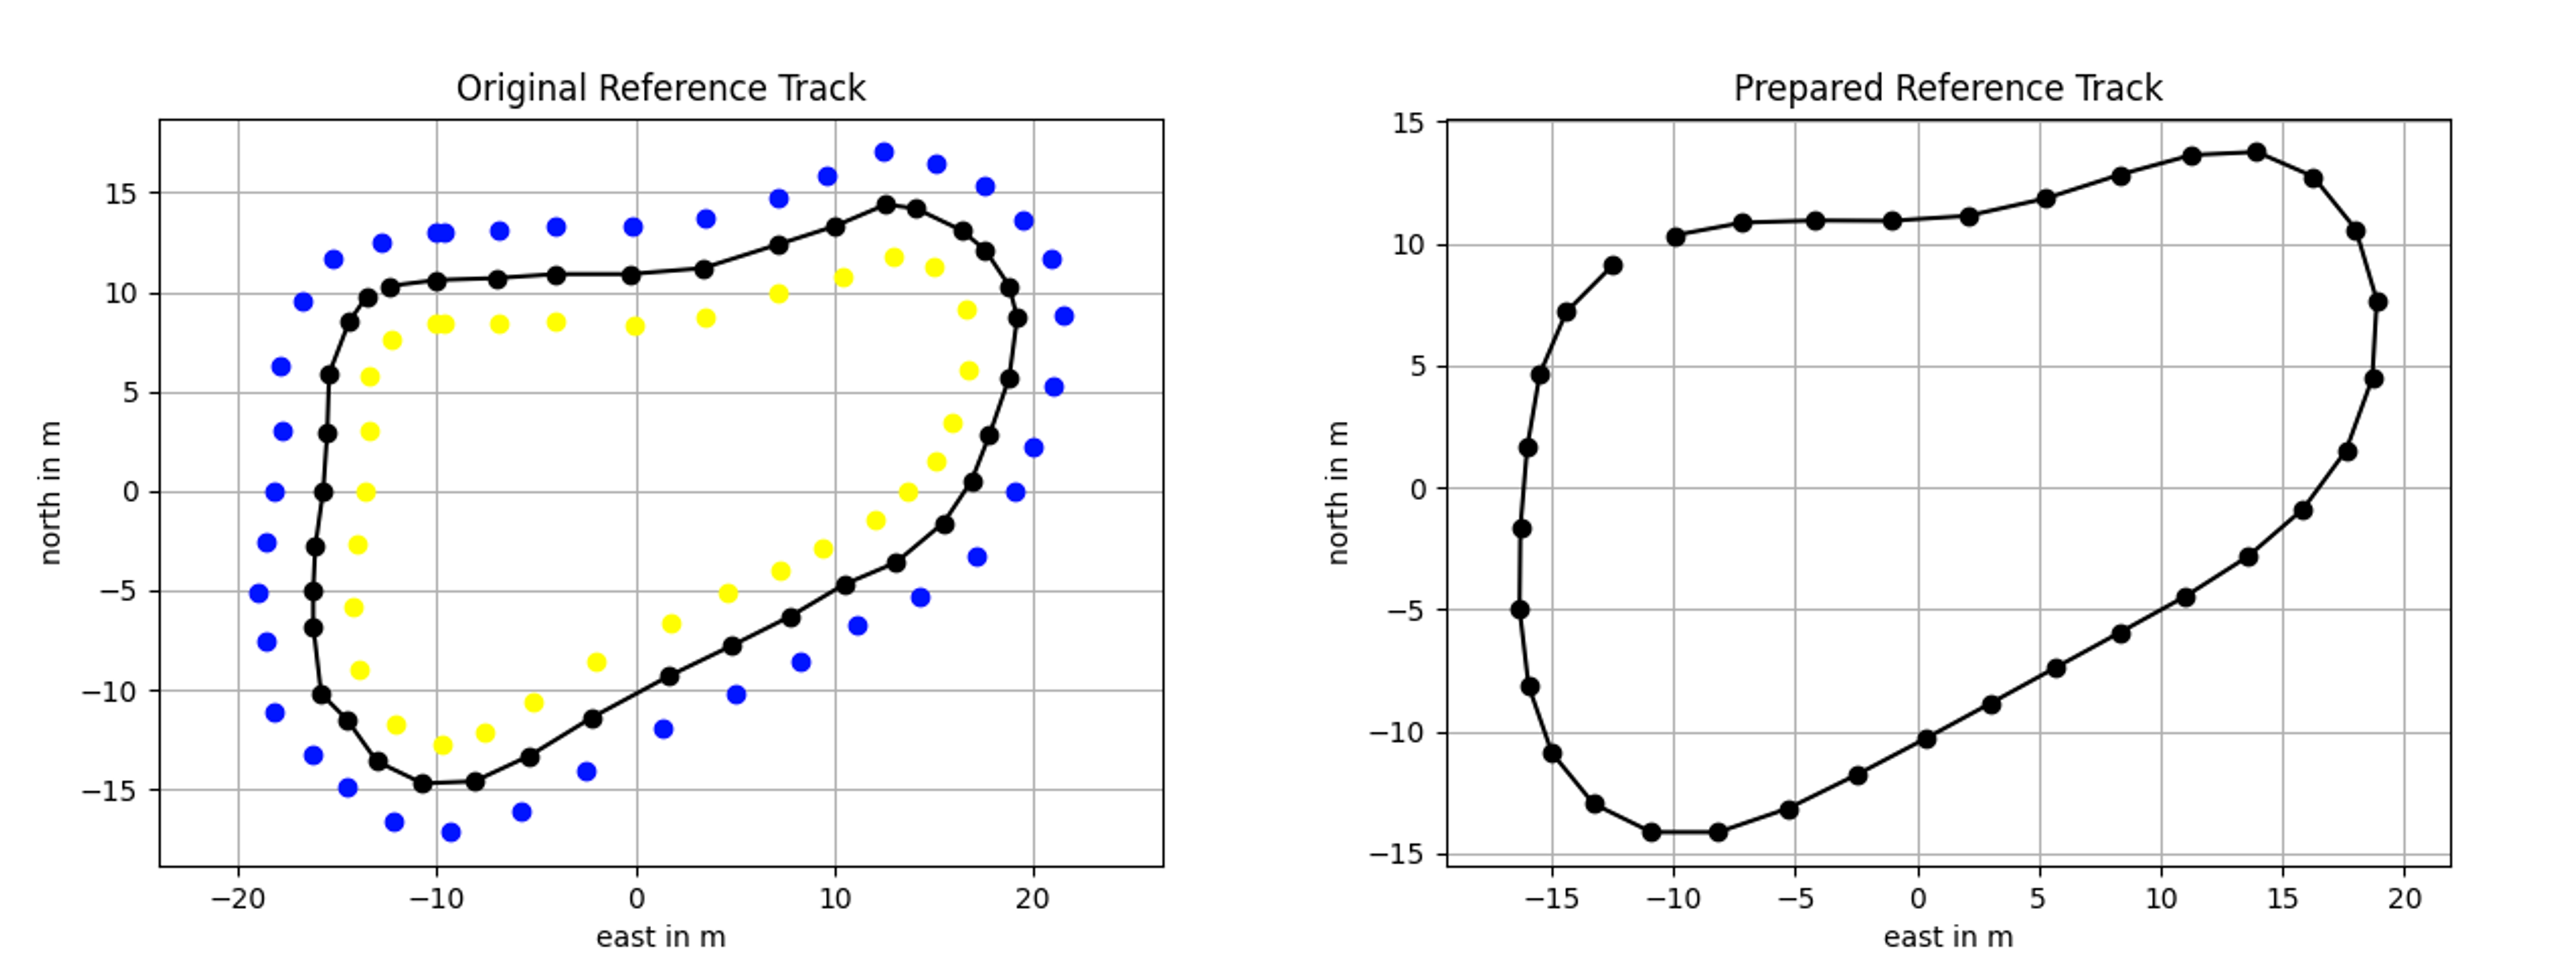
\includegraphics[width=\columnwidth]{Algorithm_Optimization_Prep_Track.png}
    \caption{Side-by-side comparison of the original reference track and the prepared reference track after the spline approximation and calculation for the ``Small Track'' test track.}
    \label{fig:Optimization Algorithm Prepare Track}
\end{figure}
To ensure a solution is possible, the normal vectors (spline normals) are checked for crossing points.
\begin{figure}[H]
    \centering
    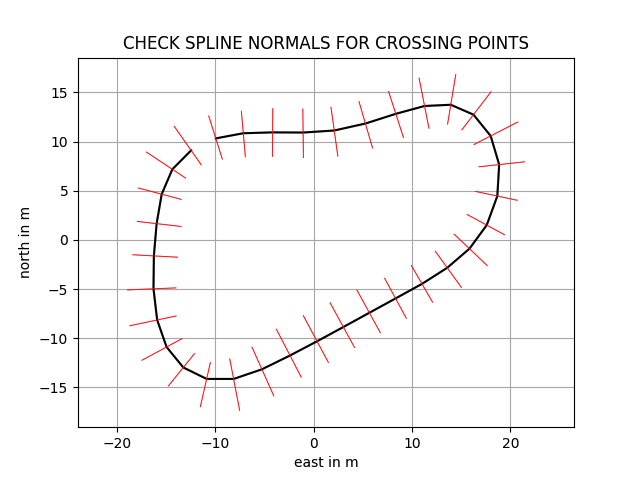
\includegraphics[width=\columnwidth]{Algorithm_Optimization_Check_Splines.png}
    \caption{Checking of the spline normals for crossing points on the ``Small Track'' test track.}
    \label{fig:Optimization Algorithm Check Spline Normals for Crossing Points}
\end{figure}
Finally, if no crossings are detected, the minimum track width set by the user is enforced by inflating tighter sections until the desired track width is reached.
\begin{figure}[H]
    \centering
    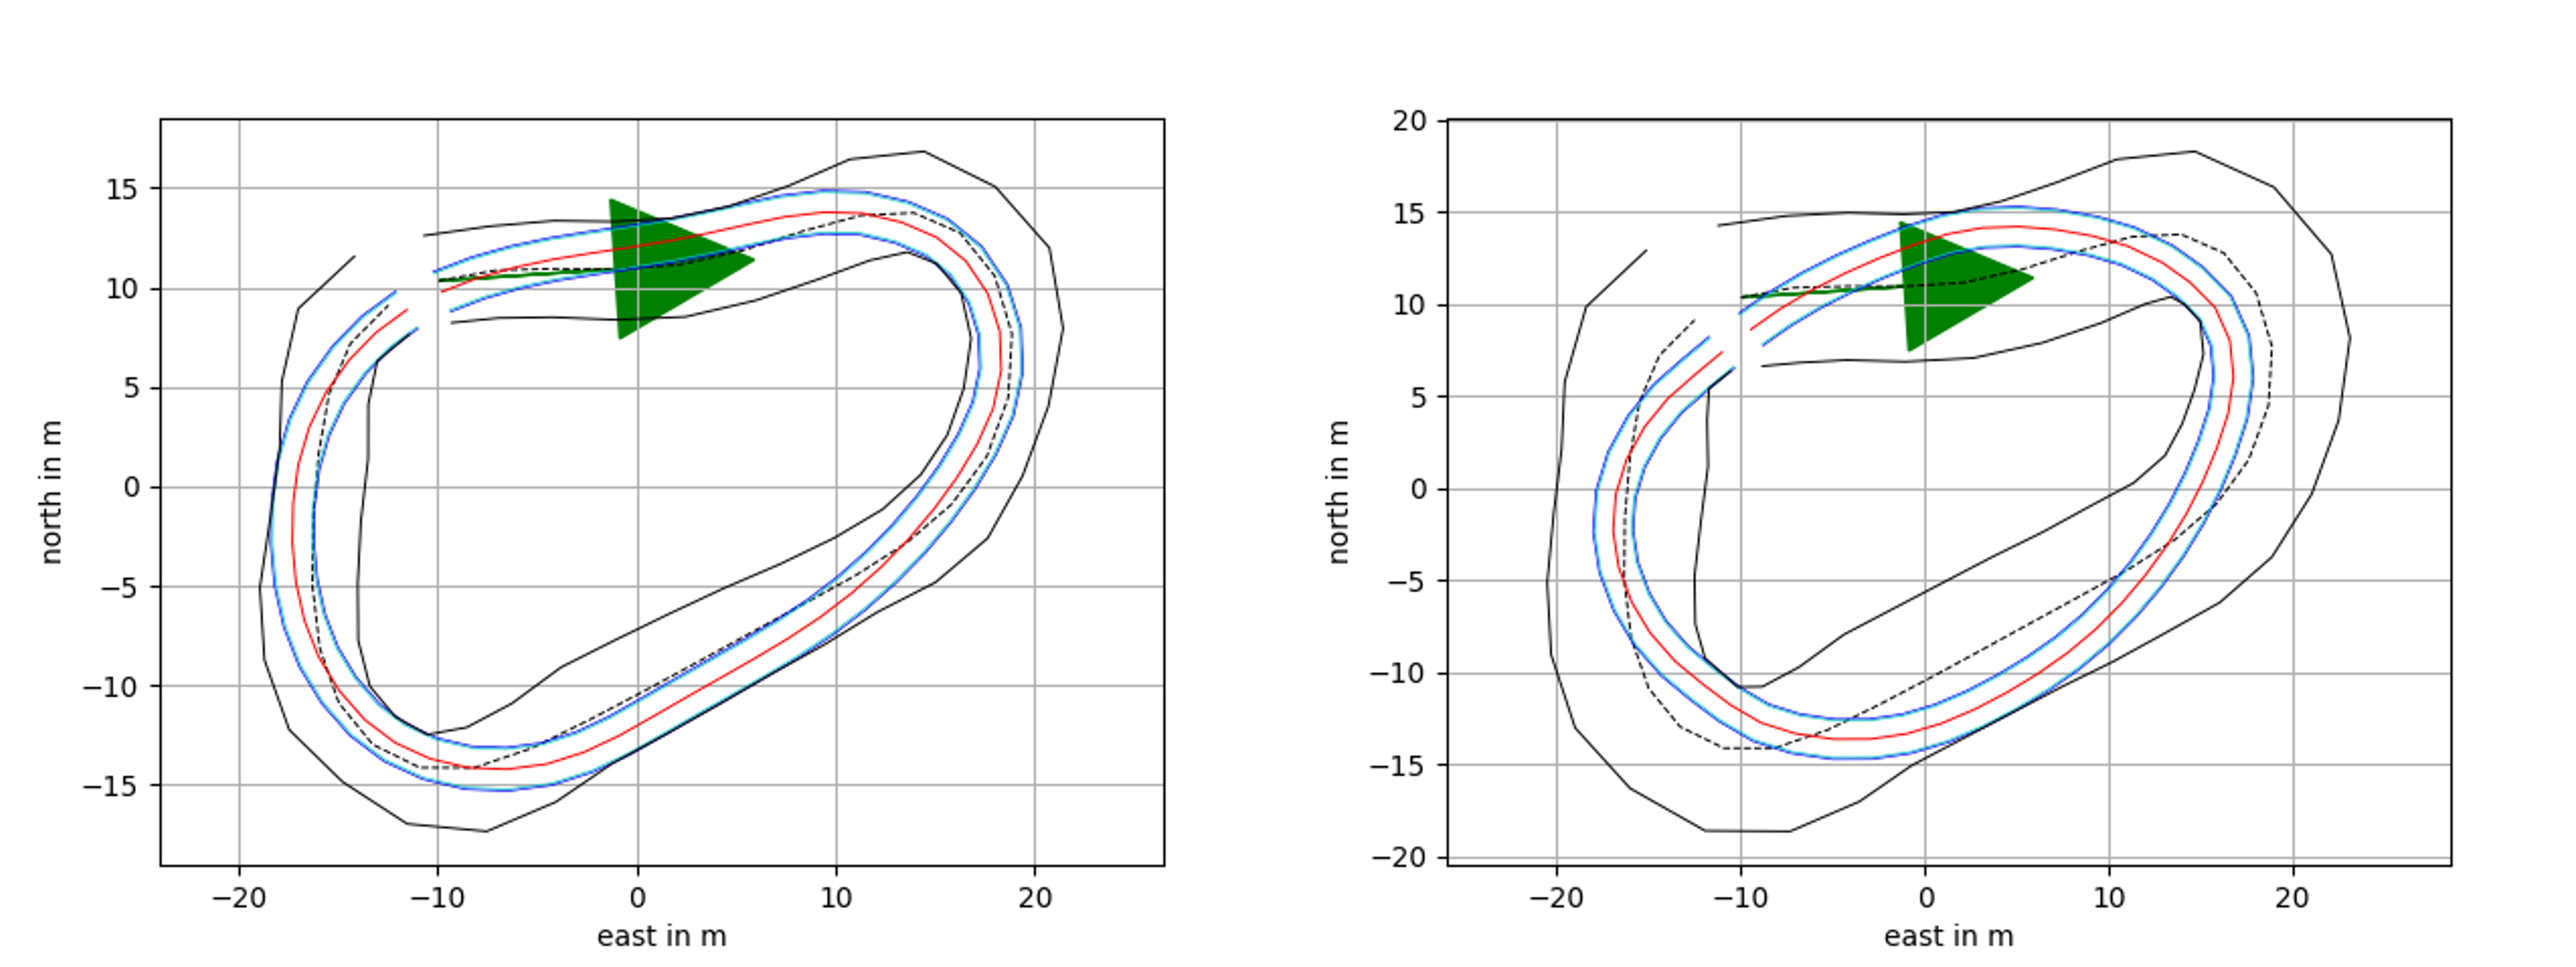
\includegraphics[width=\columnwidth]{Algorithm_Optimization_Enforce_Min_Width.png}
    \caption{Comparison of the ``Small Track'' test track with no minimum track width set (left side), and the same track with an arbitrary high minimum track width set (right side).}
    \label{fig:Optimization Algorithm Check Spline Normals for Crossing Points}
\end{figure}

\textbf{3. Call Optimization}

As next, the selected optimization objective gets called: Shortest Path, Minimum Curvature or Minimum Time objective. For each objective, the solution vector $\alpha$ of the optimization problem containing the lateral shift in m for every point will be returned.

For \textbf{Shortest Path} optimization, a QP solver is used to minimize the summed length of the path by moving the path points along their normal vectors within the track width. The algorithm is based on the paper ``Race Driver Model'' by F. Braghin, F. Cheli, S. Melzi and E. Sabbioni. \cite{shortest_path}

For \textbf{Minimum Curvature} optimization, a QP solver is used to minimize the summed curvature of the path by moving the path points along their normal vectors within the track width. The algorithm can be used for closed and unclosed tracks. For unclosed tracks the heading $\psi_s$ and $\psi_e$ is enforced on the first and last point of the reference track. Furthermore, in case of an unclosed track, the first and last point of the track are not subject to optimization and stay untouched. \cite{minimum_curvature_trajectory_planning}

For \textbf{Minimum Time} optimization, the problem is described as an optimal control problem, converted to a nonlinear program using direct orthogonal Gauss-Legendre collocation and then solved by the interior-point method IPOPT. Reduced computing
times are achieved using a curvilinear abscissa approach for track description, algorithmic differentiation using the software framework CasADi, and a smoothing of the track input data by approximate spline regression. The vehicles behaviour is approximated as a double track model with quasi-steady state tire load simplification and nonlinear tire model. \cite{minimum_time_trajectory_planning} \cite{powertrain_behaviour}

\begin{figure}[H]
    \centering
    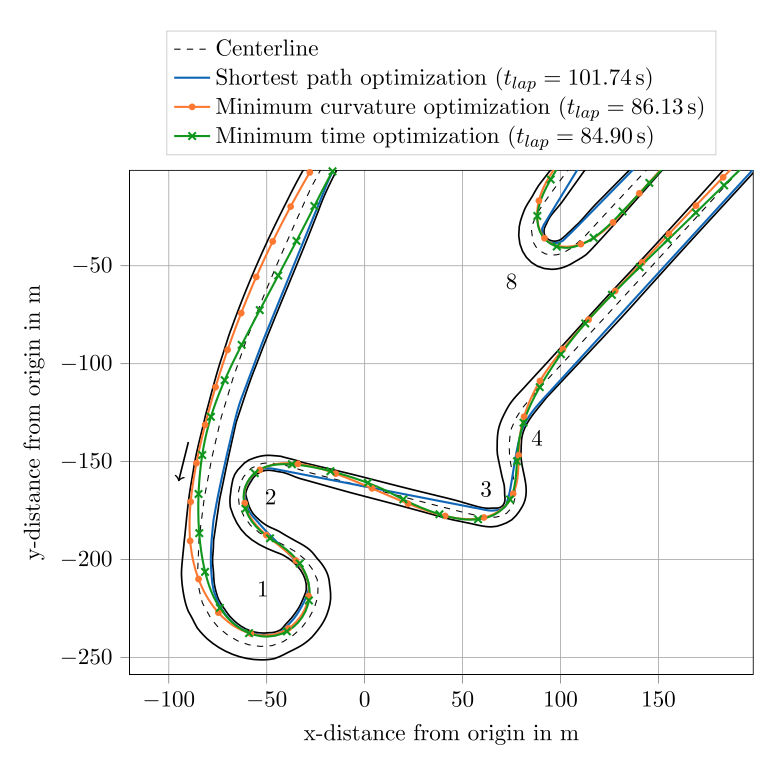
\includegraphics[width=\columnwidth]{Algorithm_Optimization_Comparison_Optimisations.png}
    \caption{Comparison of the paths resulting from the shortest path optimization, minimum curvature optimization and minimum time optimization. \cite{minimum_curvature_trajectory_planning}}
    \label{fig:Optimization Algorithm Comparing Different Optimisations}
\end{figure}

\textbf{4. Create Race Line}

After the optimization call, the race line gets created on the basis of the reference line and the optimization result by interpolating the splines to small distances between the race line points.
\begin{figure}[H]
    \centering
    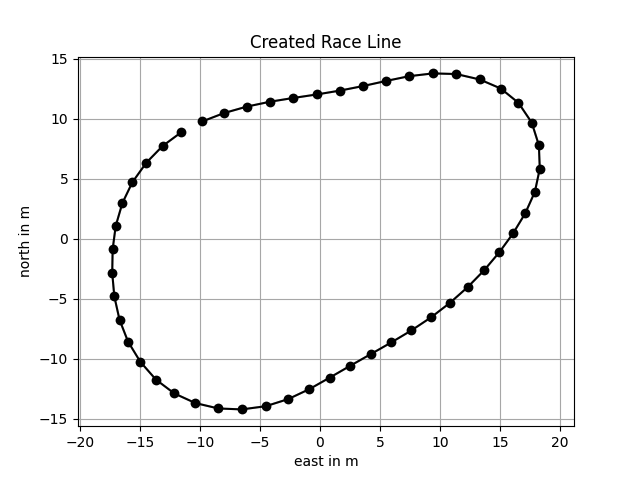
\includegraphics[width=\columnwidth]{Algorithm_Optimization_Create_Raceline.png}
    \caption{The race line created after interpolating the splines to small distances between the race line points for the ``Small Track'' test track.}
    \label{fig:Optimization Algorithm Created Race Line}
\end{figure}

\textbf{5. Calculate Heading and Curvature}

Thereafter, the analytical calculation of heading $\psi$ and curvature $\kappa$ at every point will be executed.
\begin{figure}[H]
    \centering
    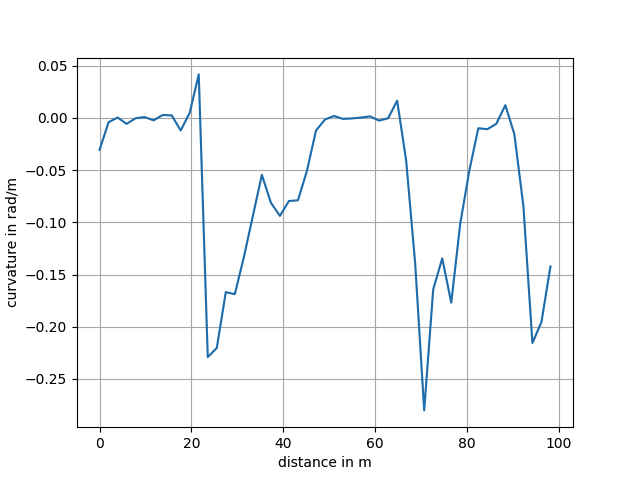
\includegraphics[width=\columnwidth]{Algorithm_Optimization_Curv_Profile.png}
    \caption{The curvature profile of the optimized path for the ``Small Track'' test track.}
    \label{fig:Optimization Algorithm Curvature Profile}
\end{figure}

\textbf{6. Calculate Velocity and Acceleration Profile}

Then the velocity profile will be created taking the tire and motor limits in consideration as good as possible. The longitudinal acceleration profile will then be created for the just created velocity profile. With both profiles, an estimated lap time gets calculated within the temporal duration (time) profile for the given trajectory.
\begin{figure}[H]
    \centering
    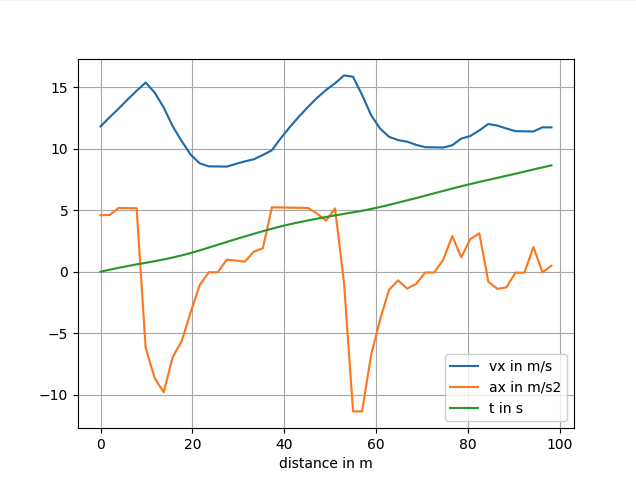
\includegraphics[width=\columnwidth]{Algorithm_Optimization_Vel_Ac_Profile.png}
    \caption{The velocity and acceleration profile for the optimized path for the ``Small Track'' test track.}
    \label{fig:Optimization Algorithm Velocity and Acceleration Profile}
\end{figure}

\textbf{7. Data Post-processing}

Lastly the data will be arranged into one trajectory and a closed race trajectory array will be created. The generated trajectory will be checked in regard to minimum distance to the boundaries and maximum curvature and accelerations. And the final trajectory gets returned and plot figures get created, if selected.

\section{Integration and Verification} \label{sec:Integration and Verification}

\begin{itemize}
    \item Tests
    \item Integration (inkl. Switch)
    \item Verifikation über Simulationstool (wie ist das setup aufgebaut, welche strecken wurden getestet)
\end{itemize}

\subsection{Visual Test with Plots} \label{sec:Visual Test with Plots}
Several test methods have been used to integrate and validate the algorithms. The first method was the visual testing of plots. Python has a library called ``matplotlib.pyplot'' which can plot points, graphs and other structures on a coordinate system. To get an idea what a good algorithm is CSV files were used for getting the track information and publish it with the ``cone\_publisher'' node. The first step was to plot the full track with the start position of the car, the yellow and blue cones and the finish line which is represented with the orange cones. The second step was to test the exploration algorithm by plotting the triangulation. After that the middle points of the edges in the simplices where calculated and plotted on the coordinate system as well. This helped to get a feeling of what a good exploration algorithm looks like. The test results are found in chapter \ref{ch:Results}. Further on the path smoothening algorithm was tested visually in the coordinate system.

For the optimization algorithm a separate node was constructed which takes a CSV file with the middle line and the distance to the border of the track. Additionally, parameters of the physics of the car can be added to have an accurate perception of how fast the car should drive and what steering angle it should turn. The split of the logic of the algorithms was made to work separately on the code. The optimization algorithm has an output of the optimized track, an acceleration profile and steering angles on each point of the optimized path. The evaluation was done by plots. The same Python library was used to get an illustration of the result on a coordinate system.

\subsection{Integration} \label{sec:Integration}
The integration was done simultaneously since it is easy to integrate a python script into \acrshort{ros}. The first step is to define a type of node as described in section \ref{sec:ROS Nodes}. Then the python script has to be implemented via the ``import'' statement so that the class described in the algorithm Python script can be used in the \acrshort{ros} node. After that the node has to define a publisher statement which published the output of the algorithm. A detailed description is found in the section \ref{sec:Path Planning Component Architecture}.
In the course of a race after the first round of using the exploration algorithm, the optimization algorithm calculates the optimum path. This is done by a switch between one to the other algorithm. Since the track has orange cones to mark the start and the end of the track this property is used to switch from one algorithm to the other. The detector of the finish line is described in section \ref{sec:Start Finish Detector}

\subsection{Verification with the Simulation Tool} \label{sec:Verification with the Simulation Tool}


